\documentclass[12pt, masters-t, a5block]{usthesis}

\usepackage[utf8]{inputenc}

\usepackage{booktabs} % For formal tables
\usepackage[]{algorithm2e}
\usepackage{url}
\usepackage{graphicx}
\usepackage{amssymb}
\usepackage{listings}
\usepackage{color}
\usepackage{amsmath}
\usepackage{setspace}
\usepackage{fancybox}
\usepackage{subcaption}
\usepackage{tabularx,rotating}
\usepackage[colorlinks = true,
            linkcolor = black,
            urlcolor  = blue,
            citecolor = blue,
            anchorcolor = blue]{hyperref}
\usepackage[thinc]{esdiff}
\usepackage{usbib}%............................. Bibliography
%\bibliographystyle{acm}%................. Auhor-year style
\bibliographystyle{usmeg-n}%................. Auhor-year style
\renewcommand{\bibname}{List of References}
\onehalfspacing
%\setcitestyle{square}

\DeclareMathOperator*{\argmin}{argmin}

\usepackage{eso-pic}%............................ Shipout commands for watermark
    \newcommand*{\WaterMark}[2][0.15\paperwidth]{%
        \AddToShipoutPicture*{\AtTextCenter{%
                \parbox[c]{0pt}{\makebox[0pt][c]{%
                    \includegraphics[width=#1]{#2}}}}}}
        

%==== TITLE PAGE ====================================================
\title{Explaining neural networks used for modeling credit risk.}

\author{Z.\ Mohamed}{Zhunaid Mohamed}

\faculty{{Faculty of Science}}

\degree{MSc (CS)}
       {Master of Science (Computer Science)}

\supervisor{Prof.\ W.\ Visser}
\cosupervisor{Prof.\ B.\ Herbst, Dr.\ M.\ Hoffman}

\setdate{12}{2020}

\SetSponsor{The financial assistance of the National Research Foundation(NRF) towards this research is hereby acknowledged. Opinions expressed and conclusions arrived at,
are those of the author and are not necessarily to be attributed to the NRF.}

%==== END TITLE PAGE ====================================================

\begin{document}

 \frontmatter
 %\WaterMark{UScrest-WM}
 \TitlePage
  \clearpage
  
 \DeclarationDate{2020/12/10}
 \DeclarationPage
  \clearpage
 
 \address{Department of Computer Science,\\
        University of Stellenbosch,\\
        Private Bag X1, Matieland 7602, South Africa.
             }
             
\begin{abstract}             
    Calculating risk before providing loans is a common problem that credit companies face. The most common solution is credit employees manually assessing the risk of a client by reviewing their credit portfolios. This can be a slow process and is prone to human error. Recently credit companies have been adopting machine learning techniques in order to automate this process, however this has been limited to linear techniques due to interpretability being a strict requirement. Neural networks could provide significant improvements to the way credit risk is modeled, however these are still seen as black boxes. In this work we compare various techniques which claim to provide interpretability into these black boxes. We also use these techniques to provide explanations on a neural network trained on synthesized credit data.
\end{abstract}
 \tableofcontents
 \clearpage

 \listoffigures
 \clearpage
 
 \listoftables
 \clearpage

 \include{frontmatter/Nomencl}
 \mainmatter



 %==== Evaluation Section ========================================================
 \chapter{Introduction}

Machine learning techniques have become widely adopted in many different domains due to its potential to produce fast and accurate results. Some of these techniques provide on par or even surpass the predictive accuracy provided by humans. It is often difficult to tell whether the techniques are correctly solving the problem or are exploiting artifacts in the data. In domains where interpretability is required for safety or legal reasons such as in medicine \cite{10.1145/2783258.2788613} where the model has to be proven trustworthy, there is often a trade off of accuracy for greater interpretability. Inherently interpretable models such as linear models where the weight coefficients can be considered an explanation or decision trees \cite{articleb} which provide explicit rules are the techniques of choice. Neural Networks which were not considered in these domains due to them being considered a \emph{black box} now have several different techniques which aim to provide interpretations into their decision making. This thesis highlights several techniques that have been used to explain the decision making of neural networks and 3 in particular will be discussed and evaluated in detail.

\section{Problem Statement} \label{sect-intro-problem}
Suppose you are approached by a real estate agency to build a model that can predict the market price of a property given its features such as \emph{size}, \emph{location}, \emph{number of bedrooms}. Now for example say your model gives a estimated worth of R1.5 million rand for the property, it is expected that a list of reasons be given as to why this property was valued as such. If we used a simple linear regression model for this, it would be as simple as extracting the weights for each feature and listing which features contributed the most to this price. However, after some experimentation you realize that the linear regression model is not accurate enough and by using modern neural networks you are able to greatly increase your accuracy. You are now faced with a problem since there is no simple way to explain what features were important in a neural network and are forced to use the inferior model in favor of interpretability.

\section{What is a neural network}
The goal of a Neural Network is to simulate the human brains ability to detect patterns within data in order to make some decision. For example given a picture of a cat with the aim at determining whether it is a cat or a dog. By distinguishing certain features such as their ears and mouth shape we as humans are able to come to the decision that it is indeed a cat. Figure \ref{fig-ff-nn} is the generic structure of a feedfoward Neural Network. Each individual circle is a \emph{neuron} which produces some real-valued activation. Sets of neurons are separated into \emph{layers} which each have a different representation of the data. The arrows which interconnect layers are called \emph{weights}. The input layer is what the Neural Networks sees as input data such as the pixels of an image of a cat. The hidden layers are internal representations of data that is learnt by the network. The output layer is the result of the decision that network has arrived at. In order to make decisions our Neural Network first has to be trained. This entails giving the Neural Network a set of samples with their corresponding \emph{correct decisions}. In the case of differentiating between cats and dogs, we may have a set of images of both cats and dogs and their corresponding labels. The weights and hidden neurons are initialized either randomly or by some algorithm. The input data is then put through the network and the produced outputs are compared to our actual outputs. The \emph{error} is calculated which is the difference between the actual and produced output and this error is propagated back into the layers of the network in order to update the weights and neurons accordingly with an algorithm called \emph{backpropagation} \cite{10.5555/65669.104451}\cite{10.5555/525960}. This process is repeated until it is decided that the error is small enough and we end up with a trained Neural Network.


\begin  {figure}[!htpb]
\centering
  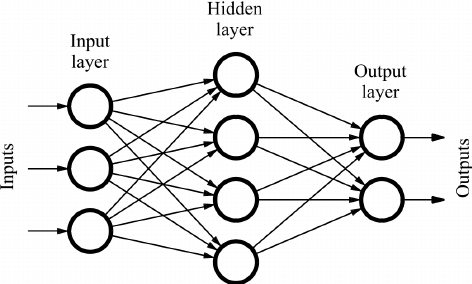
\includegraphics[width=0.9\linewidth]{Credit_Images/Sample-of-a-feed-forward-neural-network.png}
   \caption{Architecture of a generic Feedforward Neural Network \cite{inbook}.}
    \label{fig-ff-nn}
\end{figure}

\section{Why interpreting neural networks is difficult}
Neural Networks are usually treated as \emph{black boxes} of which we have little to no understanding of their inner workings. An example is present in Figure \ref{fig:panada-nn} where an adversary \cite{szegedy2014intriguing} slightly adjusted the original image on the left by generating noise which causes the Neural Network to misclassify the \emph{Panda} as a \emph{Gibbon}. From a human perspective both images are obviously of a Panda but the Neural Network was easily fooled and there is no simple way to understand why. 
\begin  {figure}[!htpb]
  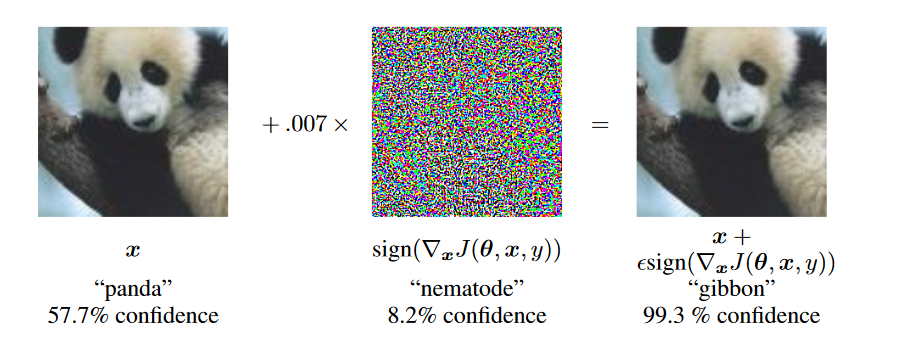
\includegraphics[width=\linewidth]{Introduction_Images/nn-unexplainable.png}
   \caption{A demonstration showing that by adding a small amount of noise to the image of a panda we were able to fool the Neural Network into misclassifying it as a gibbon \cite{goodfellow2015explaining}.}
    \label{fig:panada-nn}
\end{figure}
Looking at the architecture of a Neural Network we could identify which individual neurons activate based on the presence of certain features, an example being the shape of the pandas nose in Figure \ref{fig:panada-nn}. However, this does not seem to be true as both images contain the same features yet the Neural Network failed to correctly identify the panda. Therefore the idea of directly monitoring how neurons activate in response to features is not reliable. In the case of a linear model trained on images we could simply look at the relationship between the features extracted from algorithms such as SURF \cite{10.1016/j.cviu.2007.09.014} and SIFT \cite{Wu2013ACS} and the output. This is not as simple when working with Neural Networks due to the hidden layers having their own transformations that are learnt through backpropagating the errors \cite{10.5555/65669.104451}\cite{10.5555/525960}. In the case of a \emph{Convolutional Neural Network (CNN)} \cite{DBLP:journals/corr/Schmidhuber14} which is an image-based network, simply viewing the hidden layers may look like noise. In a CNN the features which are extracted are learnt by the network itself and may result in the reliance on noise or artifacts within the image. Another example can be seen in Figure \ref{fig:negative-nn} when changing the images to their negative the network is unable to discern the correct class. This shows that rather than specifics like edges and shapes the classifier could be relying on color specific artifacts in it's classification scheme.
\begin  {figure}[!htpb]
  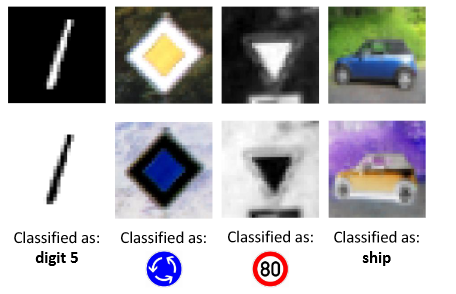
\includegraphics[width=\linewidth]{Introduction_Images/NN-negative.png}
   \caption {Simply making the images negative causes a misclassification by the network \cite{DBLP:journals/corr/HosseiniP17}.}
    \label{fig:negative-nn}
\end{figure}
It is natural to think that by providing the images altered by the noise into the training data we can prevent this form of misclassification. This is not feasible as we can not protect against every form of alteration. Therefore we need concrete explanations on how the input features affect the classification scheme of the network so that we may ascertain that the network has properly learnt actual features rather than artifacts. This extends to other network architectures. For a \emph{Recurrent Neural Network (RNN)} \cite{DBLP:journals/corr/Schmidhuber14} trained on classyfing a movie review as either good or bad, by slightly altering the input sequences it was possible to have the network misclassify 100\% of the training data \cite{DBLP:journals/corr/PapernotMSH16}. For instance changing the review “I  wouldn’t  rent  this  one  even  on  dollar  rental  night.”  into  “Excellent wouldn’t  rent  this  one  even  on  dollar  rental  night.” the network was fooled into misclassyfing the review as positive \cite{DBLP:journals/corr/PapernotMSH16}.  By simply inserting words with positive connotations into the input the RNN was mislead. The goal of providing a relationship of input features to prediction output is referred to as the \emph{attribution problem} \cite{DBLP:journals/corr/SundararajanTY17}.

\subsection{Overview of Interpretability}
As we have discussed in the previous section, linear models can be easily explained since their prediction is simply a linear combination of feature values weighted by model coefficients. However due to the need for more powerful non-linear models \emph{Random Forests} \cite{inbookb} among others  became a popular choice. Random Forests is a technique that constructs multiple decision trees and outputs the prediction as the average prediction of the individual trees. Since this technique was non-linear it was not adopted into many fields due it being difficult to interpret. A PhD thesis by \emph{Gilles Louppe} \cite{louppe2015understanding}  provided a methodology for extracting the  importance of features on a global level from Random Forests. The interpretability of Random Forests was further expanded when the popular machine learning library \emph{scikit-learn} released a blog post on how to obtain importance of features for individual predictions \cite{RandomData}. With the sudden growth in popularity of Neural Networks, interpretation was once again needed before it could replace older and weaker techniques. There have been several techniques which aim to interpret Neural Networks which range from using decision trees to approximate the network to isolating individual neurons in an attempt to explain their importance. These techniques are discussed in more detail in chapter \ref{sect-related}. For this thesis we have chosen 2 tools which claim to be model-agnostic explainers and a tool which provides a deep framework to explore the inner workings of a neural network. These will be discussed in detail in chapter \ref{sect-background}.

\section{Our approach}
\subsection{Discuss and Evaluate our chosen tools}
We discuss and evaluate 3 chosen tools which aim to provide interpretation for Neural Networks decisions. We have selected popular machine learning problems which range from the popular \emph{MNIST} digit classification problem to predicting whether a movie review posted on \emph{IMDB} is positive or negative. We have trained models with varying architectures aimed at solving these problems. Using our chosen techniques we attempt to provide explanations into these models in order to discern which features have the biggest impact in determining the prediction. We also compare how these explanations differ for different input types and whether they can be easily understood.

\subsection{Generate explanations for a Neural Network used to solve a real world credit problem}
The main contribution of this work is that we apply these techniques on a real world example. The credit space is a high risk environment and therefore any machine learning technique that is used has to be interpretable. Using a credit risk dataset provided to us we will train both a linear model, which is a commonly used solution, and a Neural Network. Using our chosen tools, we will generate explanations for the Neural Network and compare them to the inherent explanations present in the linear network. Our goal is to determine whether the explanations for the neural networks are good enough to allow them to be used for risk modeling.

\section{Thesis Goals}
The goals we are aiming to achieve with this thesis are as follows:
\begin{itemize}
    \item Evaluate the explanations between our 3 chosen tools and various machine-learning problems.
    \item Train a linear model and a Neural Network on the provided credit risk data.
    \item Provide explanations into the credit neural network and compare the interpretability to the linear model.
    \item Answer the question whether these explanations are sufficient enough to consider Neural Networks in domains where interpretability is a strict requirement.
\end{itemize}
\section{Thesis Structure}
\begin{description}
 \item[Chapter 2] describes related techniques used for providing interpretability into Neural Networks.
 \item[Chapter 3] provides a detailed background into our 3 chosen tools by thoroughly explaining their inner workings.
 \item[Chapter 4] provides an evaluation and comparison between the explanations generated by our chosen tools on various popular machine learning problems.
 \item[Chapter 5] we train and evaluate a model trained on credit risk data and provide explanations using our tools.
 \item[Chapter 6] concludes our research.
\end{description}
 \chapter{Related Work} \label{sect-related}
Our 3 chosen tools includes 2 model-agnostic explainers, namely \emph{LIME} \cite{lime} and \emph{SHAP} \cite{NIPS2017_7062}. As well as a collection of infrastructure and tools for research in neural network interpretability known as \emph{Lucid} \cite{Https://github.com/tensorflow/lucid}. These tools will be discussed in greater detail in chapter \ref{sect-background}. In this chapter we will discuss related research efforts of attempting to provide interpretability into Neural Networks and we state why we have not chosen them to evaluate.

\section{Activation Maximization}
\emph{Activation Maximization (AM)} is the idea of generating input patterns that would maximize the activation of a given hidden unit in a Neural Network \cite{simonyan2014deep}\cite{10.1162/neco.2006.18.8.1868}\cite{articlec}. Suppose we had a Neural Network which maps a input vector $x$ to a set of classes $(w_{c})$. The output layer of the Neural Network is a set of neurons which encode this as class probabilities $p(w_{c}|x)$. We can generate a prototype $x^{*}$ of a class $w_{c}$ by optimizing,
\begin{equation}
    \max_{x} \log p(w_{c}|x) - \lambda||x||^{2}
    \label{eq:am}
\end{equation}
where the rightmost term is a regularizer which prefers inputs which are close to the origin. The probabilities produced by the Neural Network are functions which have gradients \cite{10.5555/525960}. Therefore we are able to optimize \ref{eq:am} using gradient ascent \cite{DBLP:journals/corr/Ruder16}. This allows us to visualize the features that individual neurons are looking for within the input. For example given a network which attempts to discern whether an image is of a cat or dog. By using AM we theoretically should be able to discern which neurons in the network look for features of a dog such as floppy ears. However image-based networks prototypes mostly look like gray images where key points have patterns \cite{simonyan2014deep}. The prototypes produced by this optimization are mostly unnatural and therefore can not be considered reliable. One of our chosen tools Lucid further expands on this concept for image-based networks where the prototypes produced are easily understood. 

\section{Sensitivity analysis}
\emph{Sensitivity Analysis} \cite{DBLP:journals/corr/MontavonSM17} is a technique used to identify the most important input features within a model \cite{Zhou2008}. We use the model's locally evaluated gradient to calculate the relevance scores of the features as,
\begin{equation}
    R_{i}(x) = \frac{\partial f}{\partial x_{i}} \cdot x_{i}
\end{equation}
where  $x$ is the input features, $x_{i}$ is the feature at index $i$, and $f$ is the model. The Relevance score can be interpreted as the product of sensitivity (given by the locally evaluated partial derivative) and saliency (given by the input value) \cite{DBLP:journals/corr/MontavonSM17}. Therefore a feature can be considered relevant if it is present in the data and has a large impact on the gradient. This tells us that a feature is relevant in some way to the model, but it does not tell us exactly how it affects the prediction.

\section{Trepan}
\emph{Extracting Tree-Structured Representations of Trained Networks (Trepan)} \cite{Craven1995ExtractingTR} is an algorithm with attempts to extract comprehensible and symbolic representations from trained Neural Networks. This is done by inducing a decision tree \cite{articleb} which are interpretable and describes the concept represented by the network. The goal of the algorithm is to produce a decision tree which given the same input as the Neural Network produces the same results. The decisions made by the decision tree can be seen as the same decisions that the Neural Network makes. Therefore the interpretation of the decision tree can be seen as an approximate explanation of the network.  This algorithm was developed in 1996 and there are not many working examples in practice. Popular tools have opted for using linear models as approximators due to them being easier to compute. With Neural Networks having become more complex it would be interesting to investigate how this algorithm performs on modern architecture in a future experiment.

\section{BETA}
\emph{Black Box Explanations through Transparent Approximations(BETA)} \cite{DBLP:journals/corr/LakkarajuKCL17} is a model agnostic framework which aims to optimize both the fidelity to the original model and the interpretability of the explanation. BETA constructs a small number of compact decision sets which are inherently interpretable \cite{inproceedingsb}  with each set attempting to capture how the Neural Network behaves at certain parts of the feature space. The framework provides reasoning as to why a specific instance was assigned their label given their feature space. This is done by ensuring that each decision set does not overlap within the feature space which they provide their decision rules for. The framework is guided by 4 properties,

\begin{description}
    \item[Fidelity] The approximations should accurately represent the behaviour of the Neural Network in all parts of the decision space.
    \item[Unambiguity] A single deterministic rationale is provided for the prediction of every instance.
    \item[Interpretability] The approximations constructed should be able to be understood by humans.
    \item[Interactivity] The user should be able to customize the approximations based on their preference e.g. adjusting the approximation for patients within a certain age range.
\end{description}
BETA has been tested on a real-world depression diagnosis dataset with few features, with the majority being binary. It has not been tested on networks with complex architectures and many features. The code is propriety and has not been made public available, therefore we have not considered BETA as a possible tool for comparison.


\section{Structured Causal Models}
 Using the first principles of causality \cite{10.5555/1642718} \cite{DBLP:journals/corr/abs-1210-4852} a new method of providing feature attributions for Neural Networks is introduced in the paper \emph{Neural Network Attributions: A Causal Perspective}\cite{DBLP:journals/corr/abs-1902-02302}. The approach involves viewing a Neural Network as a \emph{Structured Causal Model (SCM)} \cite{10.5555/1642718} and computing the Average Causal Effect (ACE) \cite{rubin1978} of an input neuron on a given output neuron. The standard principles of causality has made this problem tractable by finding input neurons which can be considered latently joint such as inputs which were generated by the same data-generating mechanism. The work includes,
 \begin{itemize}
     \item A new methodology which  uses first principles to compute causal attribution in neural networks.
     \item  Providing better estimates and global perspective to causal effect through the use of \emph{Causal regressors}.
     \item  A strategy which can be used to adapt the methodology to high-dimensional data.
     \item Support for using the methodology on Recurrent Neural Networks.
     \item  Comparisons to a state-of-the-art gradient-based method.
 \end{itemize}
The proposed methodology only works on specific types of networks and the authors of the paper have considered it future work to adapt it to more generic networks. A large drawback of this methodology is that we need prior knowledge of the training dataset. It has not been adapted to a generic framework and thus the code would need to be manually adapted for each new model. Adapting this to a generic framework and expanding it to be used with more complex Neural Network architectures is a possible future experiment.

\section{Deep Visualization}
The \emph{Understanding Neural Networks Through Deep Visualization} \cite{DBLP:journals/corr/YosinskiCNFL15} paper introduced two novel tools which aimed to visualize the inner workings of a  Convolutional Neural Network (CNN). The first being a tool which provides visualization into the activations produced  by  each  layer  of a CNN and the second providing visualization of the features at each layer. The downside is that these tools only work on networks that were trained with an outdated Deep Learning Framework called Caffe \cite{jia2014caffe} which had it's last stable release in 2017. Lucid is built on the Tensorflow framework provides various different forms of visualizations into Image-based models and includes both of these concepts.
\section{DeepLIFT}
Deep Learning Important Features (DeepLIFT) is a tool introduced in \emph{Not Just a Black Box: Learning Important Features Through Propagating Activation Differences} \cite{DBLP:journals/corr/ShrikumarGSK16} and further expanded upon in \emph{Learning Important Features Through Propagating Activation Differences} \cite{DBLP:journals/corr/ShrikumarGK17} which assigns importance scores to the input variables of a model. The importance scores are assigned based on the difference from a \emph{reference} state which is selected based on the specific problem to the \emph{initial} state of the model. Each input is replaced by a reference value which indicates that something is lacking, an example being the presence or absence of a specific feature. Expanding this idea to Neural Networks we can assign each individual neuron a reference value which is simply the activation of the neuron given the reference input. Therefore the goal of DeepLIFT is to provide an explanation of the difference between the output of a model using its original input to the output using its referenced input. SHAP incorporates the ideas of DeepLIFT within it's own tooling, therefore there is no point for us to use DeepLIFT itself.
\section{Pixel-wise Decomposition}
In the paper \emph{On Pixel-Wise Explanations for Non-Linear Classifier Decisions by Layer-Wise Relevance Propagation} \cite{Bach2015OnPropagation} the concept of pixel-wise decomposition is introduced which aims to measure how pixels positively and negatively affect the prediction of an image-based model for a particular image. Two novel methods are introduced in the paper which provides pixel-wise decomposition namely \emph{layer-wise relevance propagation (LRP)} and a technique based on Taylor decomposition \cite{DBLP:journals/corr/MontavonBBSM15} which yields an approximation of layer-wise relevance propagation. Lucid also provides explanations for individual pixels in an image so  for our use-case pixel-wise decomposition is redundant.

\section{aLIME}
\emph{Anchor Local Interpretable Model-Agnostic Explanations (aLIME)} \cite{ribeiro2016nothing} is system which aims to explain individual predictions with if-then rules in a model-agnostic manner. The rules provided are intuitive to humans and are usually easily understood. aLIME achieves this by providing rules which ``anchor'' a prediction which means that with a high probability any other change to the instance should not have an effect on the prediction. Given a model which predicts if an adult's salary is higher or lower than \$50,000 salary. An example of an anchor would be that the model always predicts the adult to earn more than \$50,000 if they have beyond a high school education regardless of other features.  The aim is to provide the shortest anchor which has the highest precision, however it is unfeasible to exactly solve this so it does by making use of approximations. At the moment aLIME only supports explaining individual predictions for text classifiers or classifiers that act on tables. It is an open source project so it is possible for a future contributor to expand it to generic models.
 
\chapter{Background} \label{sect-background}
In this chapter we introduce the  tools which we which we have evaluated namely \emph{LIME}, \emph{SHAP}, and \emph{Lucid}. We also explain in detail how these tools provide explanations.
\section{LIME}
In the paper \emph{“Why Should I Trust You?”Explaining the Predictions of Any Classifier} \cite{lime} a tool named \textbf{LIME} \emph{(Local Interpretable Model-Agnostic Explanations)} is introduced which is a model-agnostic explainer that attempts to provide an interpretable \emph{explanation model} for any supervised learning problem. The \emph{explanation model} is represented by the following linear equation,
\begin{equation}
g(z') = \phi_0 + \sum\limits_{i=1}^M \phi_i z_{i}^{'}
\label{eq:lime-explanation}
\end{equation}
where $z^{'} \epsilon$ $\{0,1\}^{M}$ represents a simplified input which is explained in a later section, M is the number of simplified input features, and $\phi_{i}$ $\epsilon$ $\mathbb{R}$ is an attribute value assigned to each feature indicating their impact on the prediction \cite{NIPS2017_7062}.
The \emph{explanation model} is used as an approximation for our complex model and remains linear so that it is interpretable. Note that in the explanation model only the input and output layers are given explanations This means that the explanation is rather limited as we are unable to gather any information regarding the hidden layers. Suppose we have a model which takes in a list of symptoms that a patient is exhibiting and attempts to predict whether the patient has the flu or not. In figure \ref{fig:lime-process} we see how LIME takes the input features which are the symptoms of the patient and provides visual feedback where each feature is given a weight and a color representing how much they contributed towards or against the patient having the flu. Ultimately the visual feedback is given to a Doctor as a reference and they should be the one to give the final diagnosis.




\begin  {figure} [!htbp]
  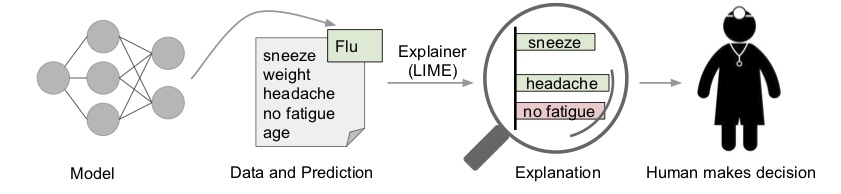
\includegraphics[width=\linewidth]{Evaluation_Images/Lime_Process.jpg}
  \caption{Example of LIME on a model that predicts whether a patient has the flu. \cite{lime}.}
  \label{fig:lime-process}
\end{figure}


\subsection{Internal data representation}Before the model can be explained, LIME performs a transformation on the input to create it's own internal representation that it can interpret. The transformation is done behind the scenes and is dependent on the type of the input data.

\begin{itemize}
\item For text data a model would commonly use complex representations such as word embeddings but a simpler representation is needed such as a binary vector where 1 indicates the presence and 0 the absence of a given word. This can be formally expressed as, 
$X^{'}={\{0,1\}}^{p}$ where $p$ is the number of words in the instance being explained. For example given a corpus of words \{The, cat, dog, jumped, leaped, over, under, the, fence\} and the input sentence  ``The dog jumped over the fence'', we could represent the input with the binary vector \{1, 0, 1, 1, 0, 1, 0, 1, 1\}.

\item For images a binary vector is used to indicate the presence or absence of super pixels in the image, where 1 indicates that the original value of the super pixel is used and 0 the pixel is set to grey which represents missing. This can be formally expressed as, $X^{'} = {\{0,1\}}$ where $p$ is the number of identified super pixels in the input image. Identifying super pixels is usually done by image segmentation algorithms such as Quickshift \cite{10.1007/978-3-540-88693-8_52}.

\item For tabular data such as matrices it is dependent on the type of data. In the case of numerical data the representation is simple enough so the identity mapping is used $X^{'} = X$. For categorical data a binary vector is once again used which can be formally expressed as $X^{'}={\{0,1\}^{p}}$ where $p$ is the number of features used by the model, 1 maps to the original category, and 0 to a different one sampled according to the distribution of the training data.
\end{itemize}
Regardless of the data type LIME creates a mapping function which transforms the internal data representation back into its original form for use when predicting on the actual model.

\subsection{Sampling from the input} Once the the input has been transformed into a internal representation, LIME begins sampling from the new input in order to create perturbed samples. The sampling process like the data transformation process is dependent on the type of input data.

\begin{itemize}
\item For text data, the sampling process involves removing uniformly at random, words from the instance. In our previous example ``The dog jumped over the fence'', some permutations that could be created from sampling would be ``dog jumped over the fence'', ``over the fence'', or ``jumped''.

\item For images, the sampling process is as simple as setting  values chosen uniformly at random in our vector to 0 therefore setting them to missing.

\item For tabular data such as matrices, it is once again dependant on whether the data is numerical or categorical. For categorical features we randomly set features to 0 so that they take random values within their category. For numerical features, the instance is perturbed by sampling from a normal distribution and doing the inverse operation of mean-centering and scaling.
\end{itemize}



\subsection{Training the explanation model} Finally the explanation model has be trained, given a prediction instance $x$, i.e. a specific feature set that predicts a specific probability under the model, after LIME has transformed the input into a internal data representation $x^{'}$ and a specified number perturbed samples have been generated. An individual perturbed sample $z$ is then reconstructed to represent an actual sample if needed. This is mainly done by setting the missing features to 0. The reconstructed input $z^{'}$ is predicted on the model and LIME records how the new prediction probabilities have changed. This is done for each perturbed sample, the more perturbed samples we use the more accurate the results are. By doing this LIME is able to explain the contribution of each feature towards the prediction.
We choose our \emph{explanation model} by using the following equation,
\begin{equation}
\xi(x) = \argmin_{g\epsilon G} L (f, g,\pi_{x} ) + \Omega(g)
\label{eq:explanation-loss}
\end{equation}
where f is the model that we are trying to explain, g is all potential explanation models, $\xi(x)$ represents the optimal explanation model, $L(f, g, \pi_{x})$ is the approximation of the difference between f and g, $\pi_{x}$ is a proximity measure between an instance z to x to define locality around x where instances closer to x are given a higher weighting, and $\Omega(g)$ is a complexity score given to current explanation model which needs to minimized . LIME defaults to linear sparse models which are given a complexity rating $\Omega(g) = 0$  as our domain for possible explanation models such as in (\ref{eq:lime-explanation}).
We can see in figure \ref{fig:lime-boundary} the linear decision boundary that LIME has learnt within a complex space. The crosses represent the perturbed sampled which were generated training the explanation model, where the bold cross is the initial input. The complex space is the models decision function and the dotted line is the linear explanation model that LIME has learnt.

\begin  {figure}[!htpb]
\centering
  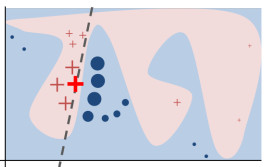
\includegraphics[width=0.7\linewidth]{Evaluation_Images/Lime_boundary.jpg}
  \caption{Linear decision function learnt in complex space.}
  \label{fig:lime-boundary}
\end{figure}



\subsection{Providing feedback to the user}
The end goal of LIME is to provide textual and visual artifacts to the end user that explains the chosen prediction. The \emph{explanation model} itself is used as the explanation for the chosen prediction. The feature attributes $\phi_{i}$ are presented to the user in a representation that is interpretable by humans.
\begin{itemize}
\item For  feedback on a image-based model, suppose we had a model which attempts to predict whether a given image is of a \emph{Electric guitar}, \emph{Acoustic guitar}, or \emph{Labrador}. In figure \ref{fig:lime-visual-feedback}, for the 3 respective classes the relevant super pixels which had a positive impact on the prediction of that particular class are displayed and the rest of the image is greyed out.
\item In the case of a model trained on text data, suppose we had a model which given an article attempts to predict whether the topic is about \emph{Atheism} or \emph{Christianity}. In figure \ref{fig:lime-textual-feedback} we can see the prediction probabilities of each class and the words which attributed towards the prediction are highlighted and given a weighting.
\end{itemize}

\begin  {figure}[!htpb]
  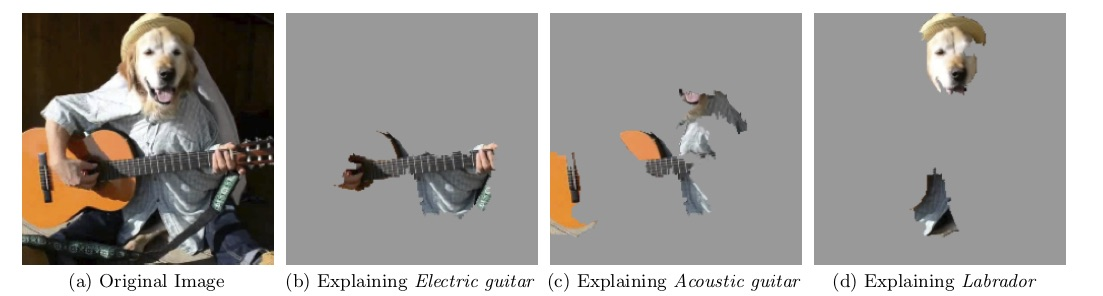
\includegraphics[width=\linewidth]{Evaluation_Images/Lime_visual_representation.jpg}
  \caption{Example of visual feedback \cite{lime}. }
  \label{fig:lime-visual-feedback}
\end{figure}

\begin  {figure}[!htpb]
  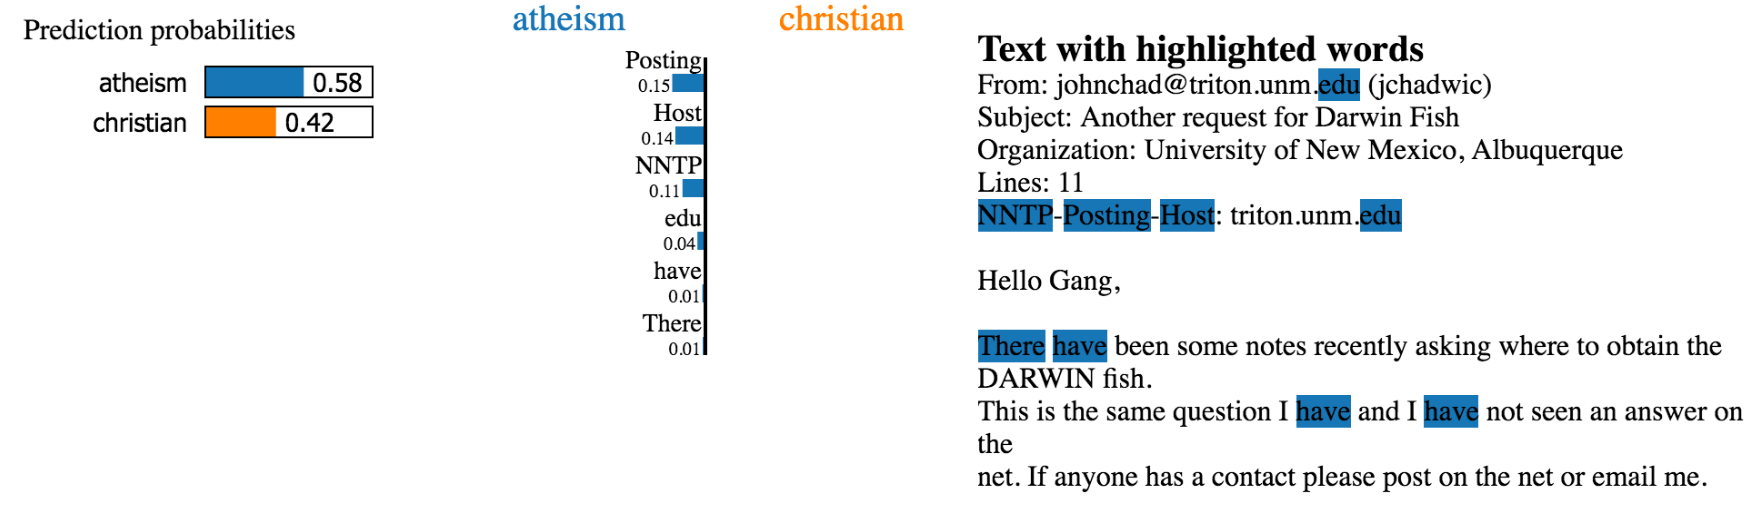
\includegraphics[width=\linewidth]{Evaluation_Images/Lime_text_represntation.png}
  \caption{Example of textual feedback \cite{Https://github.com/marcotcr/lime}.}
  \label{fig:lime-textual-feedback}
\end{figure}

\subsection{Limitations} LIME works as well as the explanation model that is built, if the explanation model does not approximate the real model well then LIME will not perform well in turn. Since LIME attempts to provide visual and textual artifacts to the user for interpretation, if there are many features such as in the thousands then even if the interpretation is accurate, a human will not be able to interpret so much information. LIME is also only able to interpret a single prediction at a time, this may not be representative of how the model performs on a global scale so it is up to the user to properly make use of this in order to gain global understanding of their model.


\section{SHAP}

In the paper \emph{A Unified Approach to Interpreting Model Predictions} a tool named SHAP(SHapley Additive exPlanations) \cite{NIPS2017_7062}  is introduced. SHAP aims to combine various different tools with LIME\cite{lime} being one of them. SHAP shows that all of these tools create the same explanation model in the form of (\ref{eq:lime-explanation}) and are called \emph{additive feature attribution methods}. The paper highlights that there is no concrete knowledge on when one method is preferable to another and how they relate, and presents a unified approach which they have named \emph{SHAP values}. SHAP then concludes that there is a single unique solution present between every \emph{additive feature attribution method} that adheres to three desirable properties that were only present in shapley value estimation methods \cite{articleb} \cite{article} \cite{inproceedings} which are among the methods that SHAP attempts to unify.

\subsection{Properties}

\subsubsection{Local Accuracy}
Requires the \emph{explanation model} $g$ to at least match the output of the original model $f$ for the simplified input $x^{'}$ (which corresponds to the original input x),
\begin{equation}
    f(x) = g(x^{'}) = \phi_{0} + \sum\limits_{i=1}^M \phi_i x_{i}^{'}
    \label{eq:accuracy}
\end{equation}
where $M$ is the number of simplified inputs and $\phi_{i}$ are their values.


\subsubsection{Missingness}
Constrains features where $x^{'}_{i}= 0$ to have no attributed impact. 

\begin{equation}
x^{'}_{i} = 0 \Longrightarrow \phi_{i} = 0
\label{eq:missingness}
\end{equation}


\subsubsection{Consistency}
 If a model changes so that some simplified input’s contribution increases or stays the same regardless of the other inputs, that input’s attribution should not decrease. Let $h_x(x^{'})$ be a mapping function that transforms a simplified input $x^{'}$ into the original input $x$, $f_{x}(z^{'}) = f(h_{x}(z^{'}))$ and $z^{'} \setminus i$ denote setting $z_{i}^{'} = 0$. For any two models $f$ and $f^{'}$, if
 \begin{equation}
    f^{'}_{x}(z^{'}) - f^{'}_{x}(z^{'} \setminus i) \geq f_{x}(z^{'}) -  f_{x}(z^{'} \setminus i)
    \label{eq:consistency}
 \end{equation}
 for all inputs $z^{'} \epsilon\{0, 1\}^{M}$, then $\phi_{i}(f^{'}, x) \geq \phi_{i}(f, x)$.
 
 \subsection{Unique solution}
 
SHAP then introduces a single unique solution which can be written as an  \emph{Additive feature attribution method} and adheres to all 3 three properties.

\begin{equation}
    \phi_{i}(f, x) = \sum\limits_{z^{'} \subseteq x^{'}} \frac{|z^{'}|!(M - |z^{'}| - 1)!}{M!}[f_{x}(z^{'}) - f_{x}(z^{'} \setminus i)]    
    \label{eq:unique}
\end{equation}
where $|z^{'}|$ is the number of non-zero entries in $z^{'}$, and $z^{'} \subseteq x^{'}$ represents all $z^{'}$ vectors where the non-zero entries are a subset of the non-zero entries found in $x^{'}$.
This equation was derived from cooperative game theory results, where the values $\phi_{i}$ are referred to as shapley values \cite{shapley1952value}. It has been proven that shapley values adhere to properties 1 and 3, but not 2. The previous \emph{additive feature attribution methods} such as LIME are proven to sometimes violate properties 1 and 3, but adhere to property 2. Thus the previous \emph{additive feature attribution methods} are adapted to use shapley values so that they adhere to all 3 properties and therefore is the solution to (\ref{eq:unique}). A new unified measure of feature importance is proposed called \emph{SHAP Values}  \cite{NIPS2017_7062} which is the solution to (\ref{eq:unique}) and is used to adapt previous \emph{attribution methods}

\subsection{SHAP Values}
\emph{SHAP Values} are the shapley values of a conditional expectation function of the original model, which means they are the solution to (\ref{eq:unique}), where $f_{x}(z^{'}) = f(h_{x}(z^{'}))) = E[f(z) | z_{S}]$, and S is the set of non-zero indexes in $z^{'}$ \cite{NIPS2017_7062}. Although the exact computation of SHAP values are challenging, by combining insights gathered from current \emph{additive feature attribution methods} it is possible to approximate them.
SHAP makes two other assumptions  \emph{model linearity} and \emph{feature Independence} in order to further simply the expected values,
\begin{equation*}
f(h_{x}(z^{'})) = E[f(z) | z_{S}],
\end{equation*}
\text{ applying our two assumptions we can simplify this as,}
\begin{equation}
\approx f([z_{S}, E[z_{\overline{S}}]])
\label{eq:summarized-unique}
\end{equation}
SHAP (SHapley Additive exPlanation) values attribute to each feature the change in the expected model prediction when conditioning on that feature.  They explain how to get from the base value $E[f(z)]$ that would be predicted if we did not know any features to the current output $f(x)$. Figure \ref{fig:shap-values} shows a single ordering. When the model is non-linear or the input features are not independent, however, the order in which features are added to the expectation matters, and the SHAP values arise from averaging the $\phi_{i}$ values across all possible orderings. \cite{NIPS2017_7062}

\begin  {figure} [!htbp]
  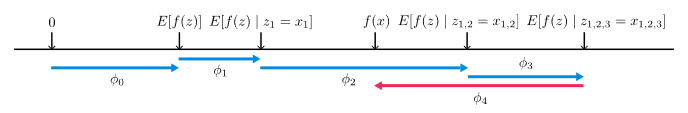
\includegraphics[width=\linewidth]{Evaluation_Images/Shap_values.png}
  \caption{How the SHAP values are computed\cite{NIPS2017_7062}}
  \label{fig:shap-values}
\end{figure}

\subsection{Types of explainers}
Using SHAP Values, the previous \emph{additive feature attribution methods} can be adapted. There are a total of 6 tools which are adapted, however in this paper we only look at the adaptions of LIME and DeepLIFT\cite{DBLP:journals/corr/ShrikumarGK17}\cite{DBLP:journals/corr/ShrikumarGSK16}.

\subsubsection{Kernel SHAP}
Adapting LIME to adhere to properties 1 and 3 which it initially violates gives rise to \emph{Kernel SHAP}, which makes use of SHAP Values. It remains model agnostic. If we refer back to (\ref{eq:explanation-loss}), we recall that $\Omega(g)$ is the term which penalizes our \emph{explanation model} based on how complex it is, $\pi_{x^{'}}$ is the locality around input $x^{'}$, and $L(f, g, \pi_{x^{'}})$ is the loss function which indicates the difference between our original model $f$ and our explanation model $g$. These three values are determined heuristically by LIME. However SHAP \cite{NIPS2017_7062} provides methods for choosing them that adheres to all three properties and has been named \emph{Shapley Kernel}.
Under (\ref{eq:lime-explanation}), the specific forms of $\pi_{x^{'}}$, L, and $\Omega$ which make (\ref{eq:explanation-loss}) consistent with the three properties of SHAP are:
\begin{align*}
   \Omega(g) = 0,
\end{align*}
\begin{align*}
    \pi_{x^{'}}(z^{'}) = \frac{(M-1)}{{M \choose |z^{'}|}|z^{'}|(M-|z^{'}|)},
\end{align*}
\begin{align*}
    L(f,g,\pi_{x^{'}}) = \sum\limits_{z^{'}\epsilon Z} [f(h_{x}(z^{'})) - g(z^{'})]^{2} \pi_{x^{'}}(z^{'}),
\end{align*}
where $|z^{'}|$ is the number of non-zero elements in $z^{'}$. $\Omega(g)$ remains 0 because we still use linear models, $\pi_{x^{'}}(z^{'})$ is the weighting of how close the sampled input $z^{'}$ is to the simplified input $x^{'}$  where $M$ is the number of features in $x^{'}$, and $L(f,g,\pi_{x^{'}})$ is the mean squared error which depends on the weighting of $\pi_{x^{'}}(z^{'})$. 


\subsubsection{Deep SHAP}
DeepLIFT was proposed as a recursive prediction explanation model for deep learning \cite{DBLP:journals/corr/ShrikumarGSK16}\cite{DBLP:journals/corr/ShrikumarGK17}. The user assigns each feature a reference value which is typically a background feature for that particular feature. For each input $x_{i}$ a value $C_{\Delta{x_{i}}\Delta{y}}$ is given which represents the effect of setting that particular input to it's reference value. Once again we introduce the mapping function $x = h_{x}(x^{'})$ that converts a simplified binary input $x^{'}$ to the original input $x$, where 1 indicates the input takes it's original value and 0 it takes it's reference value.
DeepLIFT therefore uses the following property named the ``summation-to-delta property'' \cite{NIPS2017_7062},
\begin{equation}
    \sum\limits_{i=1}^{n}C_{\Delta{x_{i}}\Delta{o}} = \Delta{o},
    \label{eq:deeplift}
\end{equation}
    where $o = f(x)$, $\Delta{o} = f(x) - f(r)$, $\Delta{x_{i}} = x_{i} - x_{r_{i}}$, and $r$ is the reference input.
    (\ref{eq:deeplift}) can be written in the form of (\ref{eq:lime-explanation}) by setting $\phi_{i} = C_{\Delta{x_{i}}\Delta{o}}$ and $\phi_{0} = f(r)$, therefore it is an \emph{additive feature attribution method}.
Although \emph{Kernel SHAP} is completely model-agnostic, we can leverage extra knowledge abut deep networks in order to increase computational performance. DeepLIFT on it's own only satisfies the local accuracy and missingness properties, but if we interpret the reference values $r_{i}$ as $E[x]$ in  (\ref{eq:summarized-unique}) then DeepLIFT approximates SHAP values and consistency is also adhered to given that the model is linear and the features are independent of one another. The new method is labeled \emph{Deep SHAP} which not only computes SHAP Values but also combines the values computed for smaller components of the network into values for the whole network \cite{NIPS2017_7062}.


\subsection{Limitations}
SHAP has a similar limitation to LIME as that it only uses the input and output of a model for interpretation and therefore no knowledge of hidden layers is achieved. SHAP also assumes \emph{model linearity} and \emph{feature independence} which is an assumption which more complex models may not adhere to.




\section{Lucid}
Lucid is a collection of infrastructure and tools for research in neural network interpretability \cite{Https://github.com/tensorflow/lucid}. Several powerful techniques such as \emph{feature visualization}, \emph{attribution}, and \emph{dimensionality reduction} have been studied for interpreting neural networks, however these techniques have been researched in isolation and there has been not been research on how these techniques may complement one another. In the paper \emph{The Building Blocks of Interpretability} \cite{olah2018the} various parts of Lucid are used in order to gain some interpretation into the hidden layers of a CNN network, the previously isolated interpretation techniques have been unified to create a rich interface. The interface that Lucid provides can be seen in figure \ref{fig:lucid-summary}, the \emph{layers} are the layers which we are able to gain insight into, \emph{atoms} are the various ways we can group our the pixels in our input images which will be explained at a later stage, \emph{content} is the type of information we can gain, and \emph{presentation} is how this information is relayed to the user.
\cite{olah2018the}

\begin  {figure}[!htpb]
  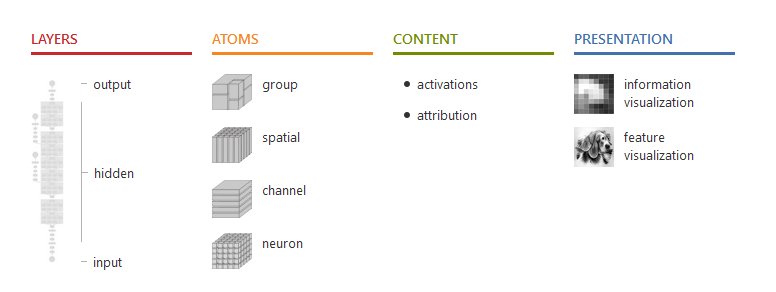
\includegraphics[width=\linewidth]{Evaluation_Images/LUCID_SUM.png}
  \caption{The interface that Lucid provides. \cite{olah2018the}}
  \label{fig:lucid-summary}
\end{figure}



\subsection{Semantic dictionaries}
The previous two tools \emph{LIME} and \emph{SHAP} only attempt to provide interpretation  between input and output layers, where as Lucid provides interpretation between any two layers. Each layer in a neural network can be seen as a three-dimensional cube where each cell represents an \emph{activation}, which is the amount that a specific neuron fires. The x- and y-axes represent the positions in the image, and the z-axes the particular channel. Usually activations are represented as abstract vectors that are not interpretable. A \emph{Semantic dictionary} is introduced which provides a more meaningful human interpretable representation of activations. \emph{Semantic Dictionaries} attempt to provide each activation with a \emph{canonical example} by mapping each activation with a visualization of that particular neuron sorted by the magnitude. This allows activations to map to similar human representations such as a ``Floppy ear'', or ``Dog snout'' when interpreting a model trained on classifying dogs. There are many ways to approximate the relationship between features and how they are used to arrive at a prediction however in this paper we linearly approximate them. 

\subsection{Types of Activations}
Since we can visualize our group of neurons as a cube, there are different ways we can slice this cube into groupings to form activations. The way each activation breaks up our cube can be seen in figure \ref{fig:lucid-maps}
.
\subsubsection{Individual Neurons}
A \emph{Saliency map} is a simple heat map which highlights pixels of a input image that cause the most output classification. Since this method works with each individual neuron we run into two big problems, each pixel in a image is usually entangled with surrounding pixels and is heavily affected by transformations such as contrast or brightness changes. The second problem is that \emph{saliency maps} are fairly limited and do not allow multiple class attributions to be displayed at one time.

\subsubsection{Spatial Activations}
Due to the limitations of the previous approach only being able to show the attributions to a single class at a time, a different approach is introduced called \emph{Spatial activations}. Spatial activations are performed from a chosen layer to all $n$-output classes. Dimensionality reduction is then performed on this n-dimensional vector to produce a multi-directional \emph{saliency map}. Once this \emph{saliency map} is overlayed on our magnitude-sized activation grid we obtain an \emph{information scent} over this attribution space. This allows attribution between layers, however different concepts are being detected together and if we continue to use spatial positions these concepts will remain entangled.

\subsubsection{Channel Activations}
By using spatial activations, the attribution is aggregated over all channels. which means we can not tell which detectors at each position most contributed to the final output classification. We can slice the cube by channels rather than spatial locations, which allows us to tell which detectors contributed the most to the output. In the case of a model which attempts to classify dogs, detectors may include those which detect ``Floppy ears'' or ``Dog snouts''.
\subsubsection{Neuron Groups}
\emph{Individual neurons} can provide the most information, however for larger networks where there may be tens of thousand of neurons this is too much information for humans. \emph{Spatial activations} and \emph{Channel activations} both provide different information about our layers, however we would gain the most if we could combine both of these techniques. There is a field of research, called \emph{matrix factorization} which studies optimal ways of breaking up matrices, we can make use of these methods by flattening our cube into a matrix of spatial locations and channels. Applying \emph{matrix factorization} on this newly created matrix, we can obtain more meaningful explanations of our layers.  By using the techniques in \emph{matrix factorization} we are able to choose what we prioritize in our activations such as describing the gradient, fully describing our activations, or if we want to fully describe the attributions. The problem with this method is that the \emph{neuron groupings} we use for a particular image can not be used for another image as each image would require a unique set of groups. 
\begin  {figure}[!htpb]
  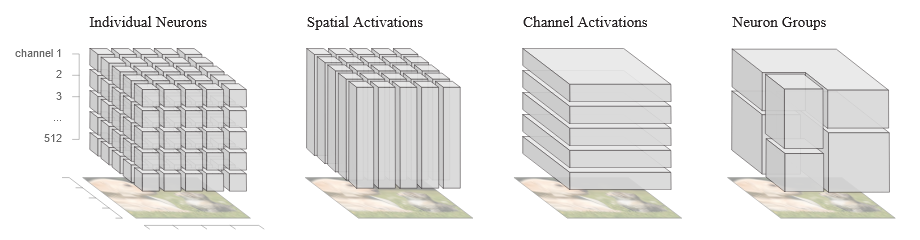
\includegraphics[width=\linewidth]{Evaluation_Images/LUCID_maps.png}
  \caption{Different types of activations. \cite{olah2018the}}
  \label{fig:lucid-maps}
\end{figure}




\subsubsection{Limitations}
Lucid is only built to be used with Tensorflow and it currently does not support the newer Tensorflow 2.0. Lucid is built on a volunteer basis and therefore there is not a lot of support on how to adapt the techniques to your domain. Since Lucid requires extensive knowledge about neural networks and interprets hidden layers, it is useful for the user who is creating the model but is not useful to the end user who has no knowledge about the architecture.

 

\chapter{Evaluation}
In this section we use LIME, SHAP and Lucid (for image-based models) on various types of models to gain an understanding on how predictions on different model architectures are explained.

\section{House Prices}
We start off by training a \emph{Random Forest Regressor} for predicting house prices as introduced in section \ref{sect-intro-problem}. We make use of the  Boston Housing Dataset which contains US census data concerning houses in various areas around the city of Boston. Each sample corresponds to a unique area and has about a dozen measures. Alongside with price, the dataset also provides information such as Crime (CRIM), areas of non-retail business in the town (INDUS), the age of people who own the house (AGE), alongside many other attributes.  The dataset contains 506 samples where the target variable is the median value of owner-occupied homes in \$1000's (MEDV).

\subsection{LIME}
Figure \ref{fig:lime-house} is the explanation LIME provides for an area in Boston where the median price of housing was predicted to be 19870\$. From this Figure we are able to deduce that the feature that had the largest negative impact on the median price of this area is the \% lower status of the population (LSTAT) and the feature which had the largest positive impact is the average number of rooms per dwelling (RM).
\begin  {figure}[!htpb]
  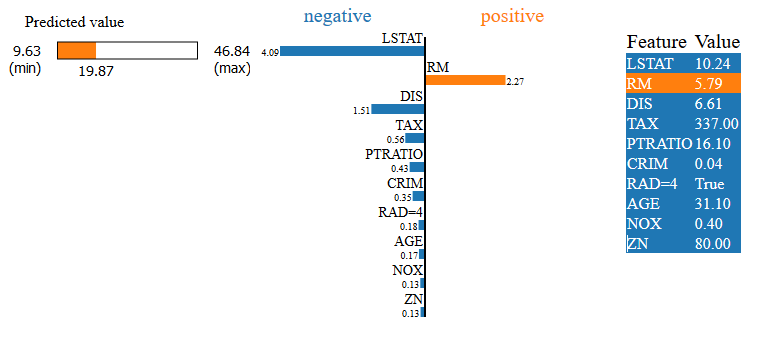
\includegraphics[width=\linewidth]{Evaluation_Images/House_LIME.png}
  \caption{LIME explanation for for a single area in Bostons median price.}
  \label{fig:lime-house}
\end{figure}
\subsection{SHAP}
Figure \ref{fig:shap-house-single} is the explanation SHAP provides for the same Boston area used in LIME. It shows features contributing to push the prediction from the base value. The base value is the average model output over the training dataset we passed. The red values have a positive impact on our prediction and the blue values a negative impact. The explanation provided is a lot different to that of LIME's, because the SHAP values represent how each feature affects the base value.
\begin  {figure}[!htpb]
  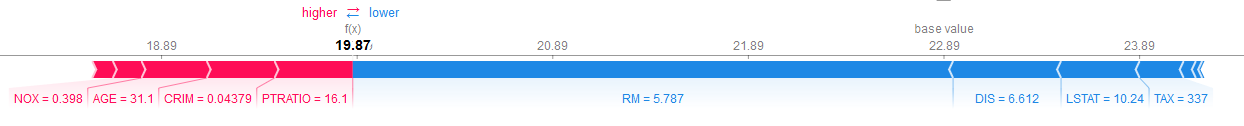
\includegraphics[width=\linewidth]{Evaluation_Images/house_indv_shap.png}
  \caption{SHAP explanation for a single area in Bostons median price.}
  \label{fig:shap-house-single}
\end{figure}
Figure \ref{fig:shap-house-entire} is the explanation that SHAP provides over multiple different areas . This is known as a summary plot and it compares SHAP values of multiple instances and how their impact on the model prediction is related to the magnitude of that feature. Features which have larger SHAP values increased the median price where as those with smaller SHAP values decreased the median price.
\begin  {figure}[!htpb]
  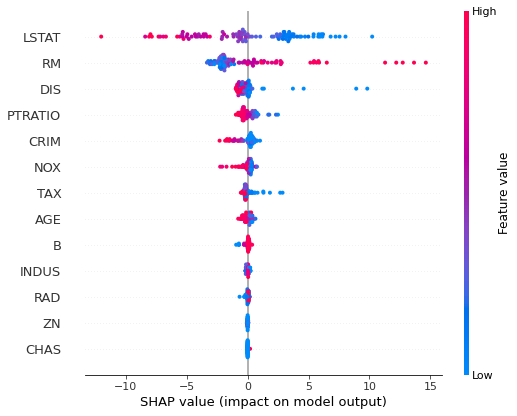
\includegraphics[width=\linewidth]{Evaluation_Images/house_shap.png}
  \caption{SHAP explanation over all the areas in Boston.}
  \label{fig:shap-house-entire}
\end{figure}
\section{MNIST}

The MNIST digit classification problem is one of the most popular machine learning problems in image processing. The dataset consists of \emph{60000} training images and \emph{10000} test images of handwritten digits with a size of $28\times28$. The goal is to determine what digit class \emph{0-9} the specific image belongs to.

\subsection{LIME}
Since there are $28 \times 28 = 784$ potential features, LIME creates a perturbed input $z^{'}$ by randomly choosing subsets of the non-zero features.  We limited the amount of samples created to 1000 for this problem. In Figure \ref{fig:lime-mnist} we can see for the specific handwritten digit \emph{5}, the green pixels represents pixels which attributed towards predicting the that the digit is 5 and red pixels which attributed towards the digit being 3.
\begin  {figure}[!htpb]
  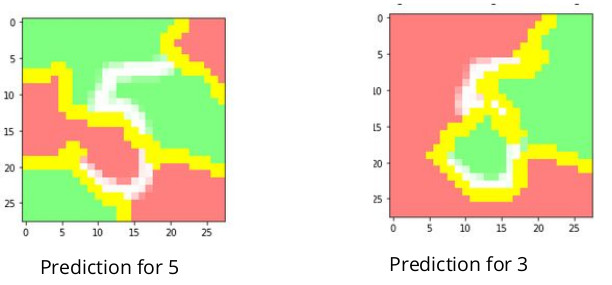
\includegraphics[width=\linewidth]{Evaluation_Images/Lime_mnist.jpg}
  \caption{Example of LIME visual feedback for the digit 5.}
  \label{fig:lime-mnist}
\end{figure}

\subsection{SHAP}
When making use of SHAP we are able to take an expectation of multiple samples in order to gain a more accurate representation of the attributed SHAP values, for this problem we took a set of 100 samples. In Figure \ref{fig:shap-mnist} we visualize our SHAP values over 4 different samples, for the 4 input images SHAP displays the SHAP values for the prediction to each class. The red masks are the pixels which attributed towards that class while the blue pixels attributed against that class.
\begin  {figure}[!htpb]
  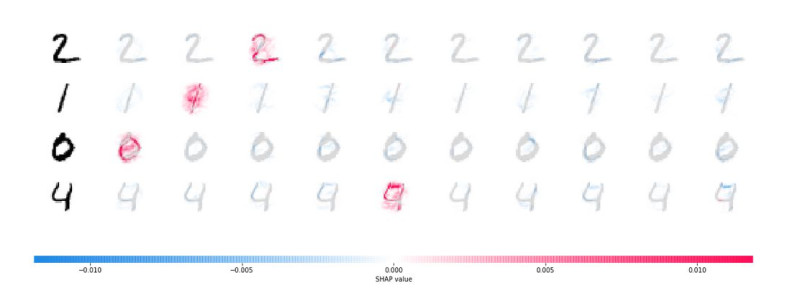
\includegraphics[width=\linewidth]{Evaluation_Images/Shap_mnist.jpg}
  \caption{SHAP values for 4 digits.}
  \label{fig:shap-mnist}
\end{figure}

\subsection{Lucid}
For Lucid we look at the spatial activations into two of our hidden convolutional layers labeled \emph{Conv2} and \emph{Conv3} respectively. Lucid provides a user interactive interface for viewing the activations, however in this example we will showcase static visual feedback. In Figure \ref{fig:lucid-mnist} for the two hidden layers \emph{Conv1} and \emph{Conv2} we are able to use spatial activations to see where and how much a specific set of pixels in the Conv1 Layer attributed in the target layer Conv2. The orange square is the set of pixels we are looking at in the starting layer and the whitened pixels in the target layer is where the activations happen

\begin  {figure}[!htpb]
  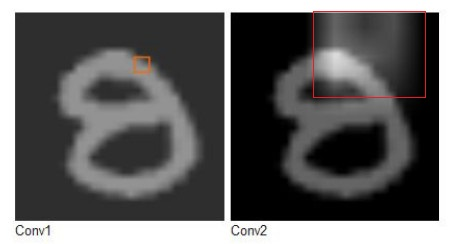
\includegraphics[width=\linewidth]{Evaluation_Images/Lucid_mnist.jpg}
  \caption{Lucid spatial activation for the digit 8.}
  \label{fig:lucid-mnist}
\end{figure} 

\section{Cats vs Dogs}

The Cats vs. Dogs is an image classification problem of finding suitable detectors for differentiating whether an image is of a cat or a dog. The dataset consists of 1000 \emph{training images} and  500 \emph{test images} with a size of $150\times150\times3$. 


\subsection{LIME}
 In Figure \ref{fig:lime-cat} we have an image of a cat and we visualize which super pixels attributed towards the \textbf{prediction of the image being a dog}, the green sections represent pixels that attributed towards being a dog where as the red sections represent pixels which attributed towards it being a cat. As a human this seems to make some intuitive sense, the ears of the cat are marked as negative attributions due to the fact that we associate dogs with ``droopy ears'', where as the cat has ``fluffy ears''.
\begin  {figure}[!htpb]
\centering
  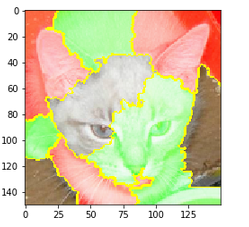
\includegraphics[width=0.8\linewidth]{Evaluation_Images/cats_explain.png}
  \caption{LIME on an image of a cat explaining which pixels attributed to it being a dog.}
  \label{fig:lime-cat}
\end{figure}

\subsection{SHAP}
In Figure \ref{fig:shap-cat} we show the SHAP values of 5 input samples and how they attributed towards whether the image is that of a cat or dog. SHAP provides much more detailed descriptions as each individual pixel is marked but LIME seems to be easier to understand as super-pixels are marked rather than individual ones. In figrue \ref{fig:shap-cat} we can see the SHAP values for 5 samples. The middle column is the attribution values for prediction towards being a cat, where as the right column is the attribution for being a dog. Red indicates a positive attribution, where as blue indicates a negative prediction.
\begin  {figure}[!htpb]
  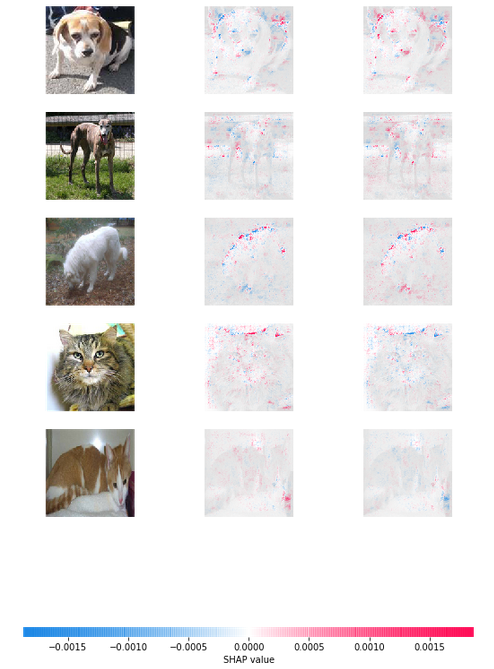
\includegraphics[width=\linewidth]{Evaluation_Images/CATS_DOGS_SHAP.png}
  \caption{Shap values for 5 different pictures of cats and dogs.}
  \label{fig:shap-cat}
\end{figure}

\subsection{Lucid}
In Figure \ref{fig:lucid-cat} we once again look at spatial activations between two hidden convolutional layers. However, in this case we included the gradient in the starting layer which shows the magnitude of the activations from the previous layers. In Figure \ref{fig:lucid-cat} for the two hidden layers \emph{Conv2} and \emph{Conv3} we are able to use spatial activations to see where how much a specific set of pixels in the Conv2 Layer attributed in the target layer Conv3. The orange square is the set of pixels we are looking at in the starting layer and the whitened pixels in the target layer is where the activations happen.
\begin  {figure}[!htpb]
  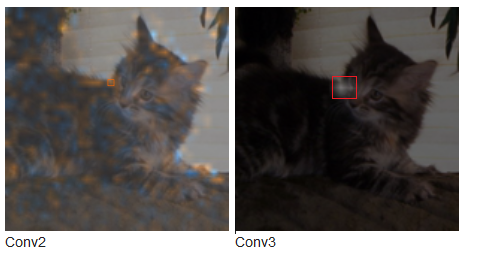
\includegraphics[width=\linewidth]{Evaluation_Images/LUCID_CATS_DOGS_2_v2.png}
  \caption{Lucid spatial activations between two layers in an image of a cat.}
  \label{fig:lucid-cat}
\end{figure}

\section{IMDB Sentiment analysis}
The goal of the \emph{IMDB sentiment analysis} problem is to classify whether a movie review is positive or negative. The dataset consists 25000 \emph{training} samples and 25000 \emph{tests sample} where is sample is a vector of size $80\times1$. Each sample is a word embedding representing which words are present and in what order.

\subsection{LIME}
In Figure \ref{fig:lime-imdb} an attribution value is given to each individual word in the review, in this example we only show 10 words which had the largest impact. Our model predicted that the review was negative, some words such as ``of'' and ``with'' by human understanding does not inherently have negative connotations, however in the context of this review it was shown that it was likely paired with negative words such as ``lies''. Due to domain knowledge being needed, there is always some human interaction and if we have thousands of words that we are attributing on, it may become difficult to understand.
\begin  {figure}[!htpb]
  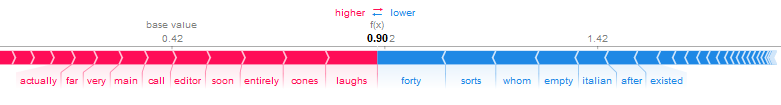
\includegraphics[width=\linewidth]{Evaluation_Images/IMDB_explanation_1.png}
  \caption{The results of the attribution where the words which had the most impact towards the prediction are sorted by magnitude. Blue represents it being a negative review and orange represents positive.}
  \label{fig:lime-imdb}
\end{figure}


\subsection{SHAP}
In Figure \ref{fig:shap-imdb} we have chosen \emph{positive} to be the primary class of prediction. In this case SHAP orders the words by magnitude of attribution and the left side indicated words that attributed towards (increased the probability) of our primary class and the right side indicates words which attributed against (decreased the probability) our primary class. Since the predicted class was \emph{negative} we can see how the negative attributions outweighed the positive attributions resulting in an output class of negative.

\begin  {figure}[!htpb]
  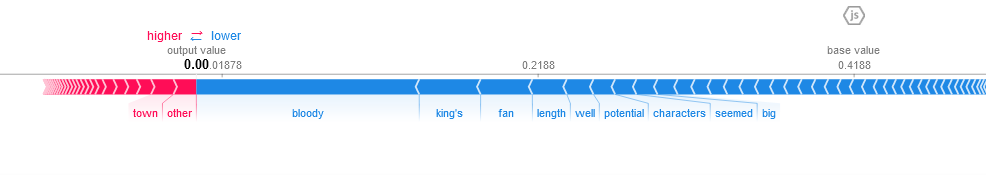
\includegraphics[width=\linewidth]{Evaluation_Images/SHAP_IMDB.png}
  \caption{The output value for this particular case was 0.00 which means we have predicted that the review is negative. The red words and words which attributed towards the review being positive, where as the blue words attributed towards the review being negative sorted by magnitude.}
  \label{fig:shap-imdb}
\end{figure}

\section{Provide intuition into LIME and SHAP}

In this section we attempt to gain intuition into LIME and SHAP by showing the relationship between a model with predefined weights and the produced feature attributions. 
\subsection{Setup}
 We start by creating a model with 5 weights which  are explicitly defined as,
\begin{align*}
w_1 = 5,\ w_2 = 3,\ w_3 = 4,\ w_4 = 9,\ w_5 = 1,
\end{align*}
in order to see the importance ratios between our weights we normalize them to unity,
\begin{align*}
    w_1 = 0.227, \ w_2 = 0.136, \ w_3 =  0.18 ,\ w_4 = 0.409, \ w_5 = 0.045.
\end{align*}
The next step is generating 500 synthetic data samples where each sample is an integer vector with 5 values between 1 and 100. We then assign each sample a probability of belonging to one of two respective classes \emph{Positive} and \emph{Negative} which are calculated as follows,
\begin{flalign*}
\begin{split}
\mbox{Sum(Positive)} &= X[0] \times w_1 + X[1] \times  w_2 + X[2] \times  w_3,
\\
\mbox{Sum(Negative)} &= X[3] \times  w_4 + X[4] \times  w_5 ,
\end{split}
\end{flalign*}
\begin{flalign*}
\begin{split}
\mbox{Prob(Positive)} &= \frac{Sum(Positive)}{Sum(Positive) + Sum(Negative)},
\\
\mbox{Prob(Negative)} &= \frac{Sum(Negative)}{Sum(Positive) + Sum(Negative)},
\end{split}
\end{flalign*}
where $X$ is the feature vector and $X[i]$ represents the feature at index $i$.
We pass this synthetic data to LIME and SHAP and observe how faithfully their produced feature attributions are to the actual weights.
\subsection{LIME}
Let $X_{1}$ and $X_{2}$ be 2 inputs with the following feature values,
\begin{flalign*}
\begin{split}
    X_1 &= [8,\ 24,\ 67,\ 87,\ 79],
    \\
    X_2 &= [48,\ 10,\ 94,\ 52,\ 98],
    \end{split}
\end{flalign*}
calculating the class probabilities for $X_1$,
\begin{flalign*}
\begin{split}
   \mbox{Prob(Positive)} &= 0.30595813,
    \\
    \mbox{Prob(Negative)} &= 0.6940418,
    \end{split}
\end{flalign*}
and for $X_2$,
\begin{flalign*}
\begin{split}
    \mbox{Prob(Positive)} &=  0.5330033 ,
    \\
    \mbox{Prob(Negative)} &= 0.4669967,
    \end{split}
\end{flalign*}
therefore $X_1$ belongs to the \emph{Negative} class and $X_2$ to the \emph{Positive} class.
We pass these two inputs to the Tabular Explainer of LIME in order to extract the feature attributions from the explanations. The visualization produced by LIME shows the feature attributions rounded to 2 significant digits, however for better accuracy our comparisons will use 3 significant digits. In Figure \ref{fig:lime-ground} we can see the attribution values which LIME assigns to each class for instance $X_1$,
\begin{align*}
    \phi_1 = 0.069, \ \phi_2 = 0.042, \ \phi_3 = 0.056 ,\ \phi_4 = 0.11, \ \phi_5 = 0.013,
\end{align*}
normalizing to unity,
\begin{align*}
    \phi_1 = 0.238, \ \phi_2 = 0.145, \ \phi_3 = 0.192 ,\ \phi_4 = 0.379, \ \phi_5 = 0.046.
\end{align*}
The explanation for $X_2$ can be seen in Figure \ref{fig:lime-ground2} and the attribution values are,
\begin{align*}
    \phi_1 = 0.061, \ \phi_2 = 0.036, \ \phi_3 = 0.048 ,\ \phi_4 = 0.126, \ \phi_5 = 0.014,
\end{align*}
normalizing to unity,
\begin{align*}
    \phi_1 = 0.215, \ \phi_2 = 0.127, \ \phi_3 = 0.167 ,\ \phi_4 = 0.441, \ \phi_5 = 0.05.
\end{align*}
\begin  {figure}[!htpb]
  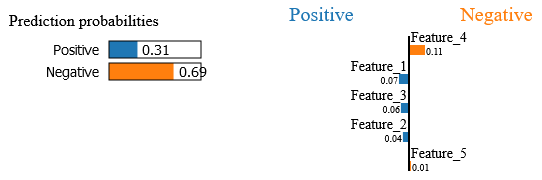
\includegraphics[width=\linewidth]{Evaluation_Images/lime-ground.png}
   \caption{LIME explanation for input $X_1$}
    \label{fig:lime-ground}
\end{figure}
\begin  {figure}[!htpb]
  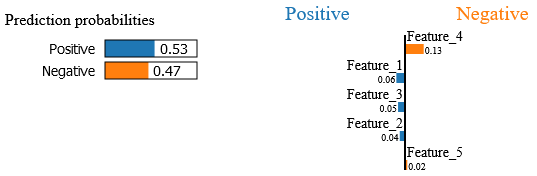
\includegraphics[width=\linewidth]{Evaluation_Images/lime-ground2.png}
   \caption{LIME explanation for input $X_2$}
    \label{fig:lime-ground2}
\end{figure}
A limitation of LIME that we have discussed before is that it only explains a single prediction at a time and we can see from the differences between the attributions values of $X_1$ and $X_2$  that there is variance between instances. This issue could be circumvented by  explaining multiple instances and averaging over the results.


\subsection{SHAP}
SHAP allows us to use our entire training set of 500 samples as background samples and gain attribution values which are averaged over the entire data set. We use \emph{Kernel SHAP} for this experiment since our model is not a Neural Network. The feature attribution values that we have derived from SHAP and normalized to unity are,
 \begin{align*}
    \phi_1 = 0.211, \ \phi_2 = 0.126, \ \phi_3 = 0.167 ,\ \phi_4 = 0.44, \ \phi_5 = 0.057.
\end{align*}
Figure \ref{fig:shap-ground} shows how each feature contributed towards the models prediction over the entire dataset for the \emph{Positive} class. The more red a point is the higher that particular feature value was, where as more blue indicates a lower value. The x-axis indicates the SHAP value, where the higher the value is the more that particular feature attributed towards the probability of the \emph{Positive} class and the lower it is the more it attributed against it. From this Figure we can see that Feature 1 to 3 attributed towards the \emph{Positive} class with Feature 1 attributing the most and Feature 2 the least. We can also see that Feature 4 attributed the most against it and Feature 5 the least. These results are inline with how we have defined our weights and from this graph we are able to visualize the different attributions between samples and their variances.
\begin  {figure}[!htpb]
  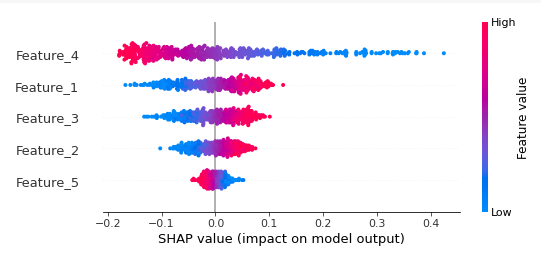
\includegraphics[width=\linewidth]{Evaluation_Images/shap_ground.png}
\caption{SHAP explanation for our chosen input $X_1$}
 \label{fig:shap-ground}
\end{figure}

\subsection{Comparison}
We have tabulated our results for comparison purposes in Figure \ref{fig:weight-tab}. We have also graphed the weights and attributions in Figure \ref{fig:weight-graph} for better visualization.We can see that the attribution values are fairly accurate in describing our defined weights and the ratios of feature importance are comparable to those of our model. From the results we have gathered, we can conclude that LIME and SHAP are able to generate fairly accurate linear estimations of a linear model by only using it's prediction results. These results allow us to gain some trust in LIME and SHAP, however further experimentation is needed to see if complex neural networks can also be approximated well.
\begin  {figure}[!htpb]
  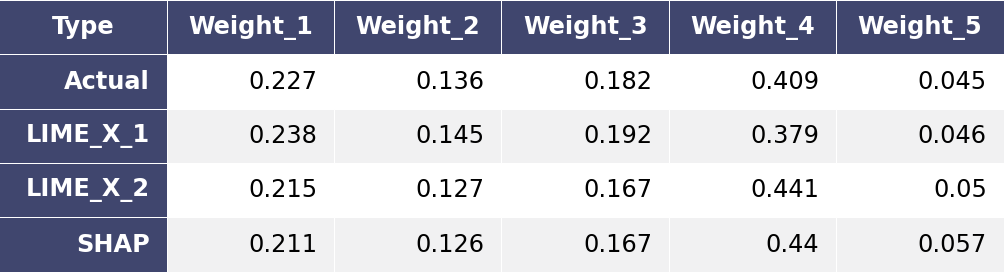
\includegraphics[width=\linewidth]{Evaluation_Images/weight_table.png}
   \caption{Comparison of weights.}
    \label{fig:weight-tab}
\end{figure}

\begin  {figure}[!htpb]
  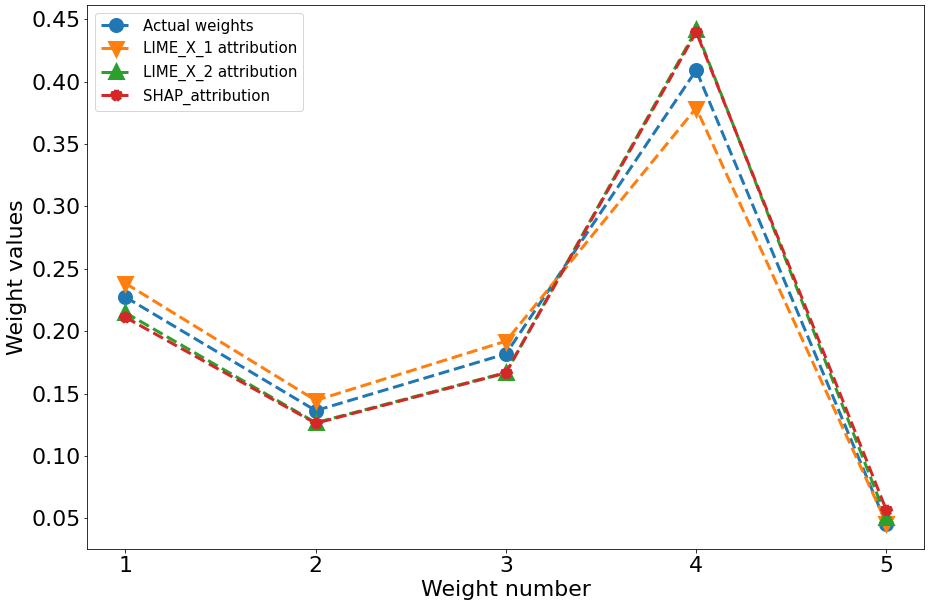
\includegraphics[width=\linewidth]{Evaluation_Images/weight_comp.png}
   \caption{Graph of weights.}
    \label{fig:weight-graph}
\end{figure}




 
%% Include weights of evidence example! Can make reference to the white paper.
\chapter{Credit Case Study}

\section{Problem Statement}
Companies which operate in the credit environment want to see returns on their investments. Before a loan is granted to a prospective client the appropriate risk analysis needs to be performed. In many instances this is a manual process where a credit employee has to assess a clients credit portfolio and ascertain if they are eligible for a loan and if so, on what terms. As most manual processes it can be slow and prone to human-error. By adopting machine-learning we are able to eliminate the human risk factor and significantly increase the speed. Linear modelling techniques such as \emph{Logistic Regression} are the preferred choice due to them being inherently interpretable. Interpretability is a strict requirement due to the need to understand why the model is making the decisions that it does. Linear models are however very limited in what they can do and by using Neural Networks or other nonlinear models we may be able to significantly increase the accuracy at identifying risk, however such techniques are generally seen as a \emph{black-box}. In this Chapter we use SHAP in order to gain some interpretability into credit risk Neural Networks so that they could be considered as possible solutions.

\section{The Data set} Up until this point we have used our tools on \emph{toy} examples where the data has been engineered to work well with machine-learning. In this Chapter we will be using a proprietary credit risk dataset which has been provided to us by \emph{Praelexis} which aims to simulate actual features used by credit companies to calculate potential client risk. Our dataset consists of a total of $200000$ client samples where $28768$ defaulted on their loan and the remaining $171232$ did not. As we can see we have a heavy class imbalance in the data with a ratio of roughly $85:15$. In practice this ratio of imbalance can be a lot higher \cite{doi:10.1142/9789812813312_0009}. The trained model may be skewed to more likely predict the most present class. How we solve this issue is discussed in Chapter \ref{sec-class-imbalance}.

\section{Aim}
 Our aim is to see if we can provide enough interpretability into a credit Neural Network so that it may be considered as a possible alternative to linear models by credit companies looking to adopt machine-learning. In order to achieve this we train a \emph{Logistic Regression} model which is inherently interpretable and a generic feedfoward Neural Network and compare their interpretability. The goal of these models is to predict a probability that a client will default on a loan given their input features. As we have seen in Chapter \ref{sect-evaluation}, SHAP is superior to LIME in every way but speed and therefore we shall use SHAP as our preferred tool for interpretation.
 
\section{Weights of evidence}
 The weights-of-evidence (WOE) transformation \cite{Siddiqi2005CreditRS} is a nonlinear transformation of the original variables. It is used to measure the strength of each attribute at separating good and bad loans. It can be seen as the measure of the difference in the proportioning of good and bad within each attribute (i.e., the odds of a person of that attribute being good or bad) \cite{Siddiqi2005CreditRS}.  Continuous variables are first converted to categorical variables through a process called \emph{binning}. Using the information from the training data we calculate the WOE value for each bin. Each client is either considered to be good (0) or bad (1).
 The WOE can be calculated as,
  \begin{equation}
     \mbox{WOE} = \left[ \ln{\left(\frac{\mbox{Distr Good}}{\mbox{Distr Bad}}\right)} \right] 
     \label{eq:woe}
 \end{equation}
The steps of calculating WOE can be therefore be summarized as follows:
\begin{enumerate}
    \item If the variable is continuous separate the data according to the distribution into multiple parts known as \emph{bins}.
    \item Calculate the number of good and bad loans in each bin.
    \item Calculate the $\%$ of good and bad loans in each bin. 
    \item Calculate the WOE of each bin by using (\ref{eq:woe}).
    \item Replace the raw variable values in the input with the WOE value of the bin that it belongs to.
\end{enumerate}
We can see an example of creating WOE bins for a variable  in Table \ref{table:woe}. The \emph{boundaries} are the bin ranges and can either be manually or automatically chosen. The \emph{Distr good} and \emph{Distr bad} is extracted from the training dataset and by using (\ref{eq:woe}) we are able calculate the WOE value for each bin. For example suppose that our input variable has a value of $1.5$. Therefore it falls into the $(1,2]$ bin and the value $1.5$ will be replaced with the WOE value $-0.07$. In Figure \ref{fig-woe-binning} we can see an example of WOE binning for a binary classifier. The axis are the values of the two features. The red star and blue dot represent the 2 classes. The shaded parts are the values which will be assigned to the 2 classes after the WOE transformations. This illustrates how the WOE transformation allows us to construct a nonlinear decision boundary.

 \subsection{Benefits of WOE}
 \begin{itemize}
     \item Missing values are separated into their own bins and is therefore easier to handle.
     \item Provides a linear relationship with log odds.
     \item It can treat outliers. Extreme values which fall outside the average range are given their own bin.
     \item We are able to determine the stability of our model by comparing the WOE values of the training and unseen data.
     \item Converts continuous variables into categorical variables so that there is no distinction between them.
 \end{itemize}
 For our dataset we have chosen to use \emph{automatic binning} because we want the preprocessing steps to be as automated as possible. This is to prevent our domain knowledge from affecting the produced explanations.
 
 

 
 \begin{table}[h!]
 \scriptsize
\begin{center}
\shadowbox{\begin{minipage}[t]{0.95\textwidth}%
    \begin{tabular}{cccccccc}
       & Bin  &  Boundaries & Count good & Distr good & Count bad & Distr bad & WoE\\
       \hline\\
       & $1$ & $(-\infty,1]$ & $1760$ & $0.0973$ & $798$ & $0.2033$ & $-0.37$ \\
       & $2$ & $(1,2]$ & $5238$ & $0.2896$ & $1 223$ & $0.3116$ & $-0.07$ \\
       & $3$ & $(2,3]$ & $7881$ & $0.4357$ & $1 034$ & $0.2634$ &  $\phantom{-}0.50$ \\
       & $4$ & $(3,\infty)$ & $3210$ & $0.1775$ & $870$ & $0.2217$ & $-0.22$ \\
        \hline
    Total & &  & $18 089$ & $1.0$ & $3 925$ & $1.0$ & 
    \end{tabular}
    \end{minipage}}
\par\end{center}
\caption{WOE example}\label{table:woe}
\end{table}

\begin  {figure}[!htpb]
\centering
  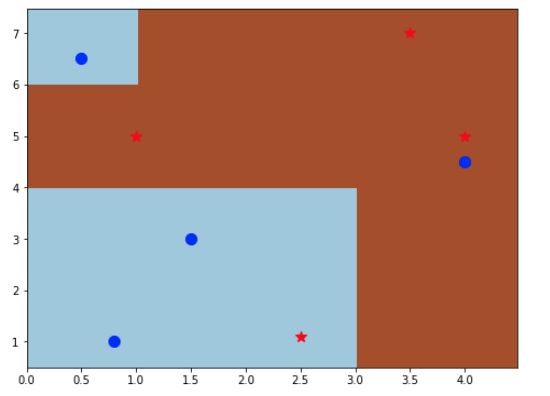
\includegraphics[width=\linewidth]{Credit_Images/WOE_EXPLANATION.png}
   \caption{Weights of evidence binning.}
    \label{fig-woe-binning}
\end{figure}

 



\section{Metrics}
Before we discuss our models architecture we introduce the metrics with which we use to measure the performance of the model. Firstly we introduce some terminology used within the metrics definitions. To provide some context we will be using our problem of predicting whether a client will default on their loan or not. We refer to clients which will default on their loan as \epmh{defaulting clients} and those which will not default as \emph{regular clients}. Defaulting clients that have been correctly identified by the model are referred to as \emph{True Positives (TP)}, where as regular clients which are incorrectly identified as defaulting clients are referred to as \emph{False Positives (FP)}. Regular Clients which are correctly identified are referred to as \emph{True Negatives (TN)}, where as defaulting clients which are incorrectly identified as regular clients are referred to as \emph{False Negatives (FN)}.
\subsection{Accuracy}
 In most examples the common metric that is used to measure how well a model performs is the \emph{accuracy} measure, however it does not work as well if the dataset has a class imbalance. Suppose in the previous example of identifying fraudulent claims that the training dataset consisted of 95\% legitimate claims and 5\% fraudulent claims. If we engineer the model to simply predict every claim to be legitimate then we will achieve a 95\% accuracy, however the model would never be able to identify fraudulent claims and therefore does not solve our problem. Although a high accuracy does not necessarily mean a model is performing well, a low accuracy can be indicative of a poor performing model and therefore has relevance. Using the previously defined terms we can define accuracy as,
\begin{equation}
    \mbox{Accuracy} = \frac{TN + TP}{FN + FP + TN + TP}
\end{equation}
\subsection{Precision}
An important metric is called \emph{precision} which is the proportion of positive identifications that were actually correct. In the previous example of identifying fraudulent claims, precision would be the percentage of \emph{actual} fraudsters in the group of people that the model has predicted to be fraudsters. Therefore using this measure we are able to determine the ratio of how many of our regular clients we have falsely predicted to be a fraudster. We define precision as,
\begin{equation}
    \mbox{Precision} = \frac{TP}{TP + FP}
\end{equation}
\subsection{Recall}
\emph{Recall} is similar to precision in that it is the proportion of actual positives that were identified correctly. In the example recall would be the percentage of fraudsters the model was able to find in the entire \emph{pool} of fraudsters. Therefore we define recall as,
\begin{equation}
    \mbox{Recall} = \frac{TP}{TP + FN}
\end{equation}
\subsection{Trade offs}
Although precision and recall both seem like metrics that we should aim to maximize in our model, in practice it is usually not possible. We have to select the metric which is most valuable to us based on the problem and use that as the performance measure while keeping the others in mind. In the case of our model which detects defaulting clients we have to weigh whether marking regular clients as defaulting clients (Precision) or identifying less actual defaulting clients overall (Recall) is more detrimental to our business. A possible solution is assigning a cost to each error made in our predictions in order make more informed decisions.
\section{Preprocessing}
\subsection{Feature Standardization}

Before we begin training our model we first have to \emph{standardize} the features. This entails subtracting the mean and scaling to unit variance so that the standardized data has a mean($\mu$) of 0 and a standard deviation($\sigma$) of 1,
\begin{equation}
    X_{standardized} = \frac{X-\mu}{\sigma}
\end{equation}
This is needed so that features have a variance within the same magnitude, because if one feature has a variance magnitudes larger than others it might dominate the objective function and in turn make the estimator rely too much on it and unable to learn from other features. 
\subsubsection{Effect on feature attributions} Standardizing the values changes their meaning to how far they are from the mean in terms of standard deviations. This means it is possible for strictly positive features to take on negative values when standardized. We have to account for this when observing the explanations.
\subsubsection{Weights of evidence}
For the WOE models the distributions of good and bad are used, which is already a form of standardization. Therefore we only perform explicit feature standardization for the raw input models.
\subsection{Splitting the dataset}
Before we start using the data we first have to split the dataset into 3 isolated sets namely \emph{training set}, \emph{validation set}, and \emph{test} set. The test and validation set will each encompass 20\% of the total data and the training set the remaining 60\%. The training set is what we use for training the model, the validation set is used to fine-tune any parameters specific to the model such as the regularizer coefficient which we will discuss in the  next Section, and the test set is only used at the end in order to evaluate the models performance on unseen data. Since we have a heavy class imbalance in the dataset, we use a \emph{stratified} split which allows each of the 3 sets to maintain the ratio of class imbalance present in the overall dataset.
\subsection{Feature Selection}
Since there are 33 features present in the dataset, we look to reduce the number of features by carefully removing those which are better explained by other features or add nothing of value to the model.  For the model which uses the raw features we will make use of a simple linear classifier with an L1 penalizer for feature selection. Since by default L1 regularization is able set weight coefficients to 0 we are able remove weights which have little or no contribution to the model. For the WOE model, we will be using Information Values extracted from the WOE for feature selection.

\subsubsection{Benefits of feature selection}
\begin{itemize}
    \item Decreased training time.
    \item More stability if correlated variables are removed.
    \item Improve the classification scheme by removing low contributing features.
    \item Explanations provided by SHAP are easier interpreted due to less features needing to be explained.
\end{itemize}

\subsubsection{Information value}
 The Information Value (IV) \cite{Siddiqi2005CreditRS} of a variable can be considered as the total predictive strength of the variable and is an indication of that variable’s ability to separate between good/bad loans. It can be seen as the symmetric alternative to the \emph{Kullback-Leibler (KL) divergence} \cite{kullback1951information}. The IV can be calculated using the following formula,
 \begin{equation}
    \mbox{IV} =  \sum^{n}_{i=1}(\mbox{Distr Good}_{i} - \mbox{Distr Bad}_{i}) \cdot \mbox{WOE}_{i}
 \end{equation}
 substituting the equation for WOE from (\ref{eq:woe}),
 \begin{equation}
     \mbox{IV} = \sum^{n}_{i=1}(\mbox{Distr Good}_{i} - \mbox{Distr Bad}_{i}) \cdot \ln{\left(\frac{\mbox{Distr Good}}{\mbox{Distr Bad}}\right)}_{i}
 \end{equation}
 where the sum is taken over all bins $n$.
 A good indication of how the IV of a variable relates to their predictive strength is shown in table \ref{table:iv}.
 \begin{table}[h!]
\begin{center}
\shadowbox{\begin{minipage}[t]{0.4\columnwidth}%
    \begin{tabular}{cl}
       \textbf{IV range}  &  \textbf{Interpretation}\\
       \hline\\
        $<0.02$ & Not predictive\\
        $[0.02,0.1)$ & Weak predictive\\
        $[0.1, 0.3)$ & Medium predictive\\
        $[0.3,0.5)$ & Strong predictive\\
        $>0.5$ & Suspicious \\
    \end{tabular}
    \end{minipage}}
\par\end{center}
\caption{IV Interpretation}\label{table:iv}
\end{table}
By calculating the IV of each of the features we are able to keep features within a certain threshold and remove the rest. For our case we have chosen the minimum threshold as $0.02$ and maximum threshold as $0.6$. Looking at Figure \ref{fig-IV-Thresh} we can see the IV of all the features and which features have been chosen to be excluded and included according to our thresholds. We have decreased the number of features from $33$ to $22$.

\begin  {figure}[!htpb]
\centering
  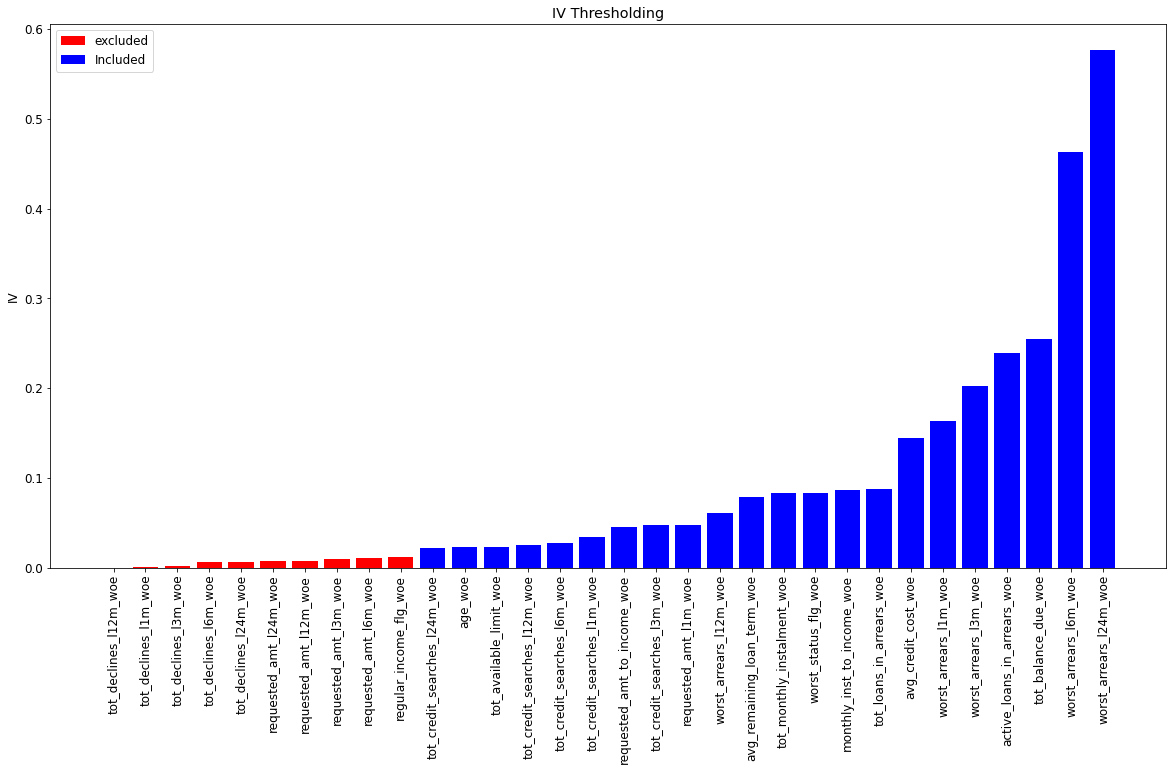
\includegraphics[width=\linewidth]{Credit_Images/IV.png}
   \caption{Information Value Thresholding.}
    \label{fig-IV-Thresh}
\end{figure}

\subsubsection{L1 Regularizer} For the raw features we use a model trained with a L1 regularizer which is referred to as a \emph{Lasso} model for feature selection. L1 regularization is able to assign higher weighting to features which play a larger role in classification and in turn can set those that do the least to 0. 
Given a linear model,
\begin{equation}
Y = \beta_{1}x_{1} + \beta_{2}x_{2} + ... + \beta_{0},
\end{equation}
where $Y$ is the label, $x_{i}$ are the features and $\beta_{i}$ are the weight coefficients.
The cost function can be written as,
\begin{equation}
\sum_{i=1}^{m}(Y_{i} - \sum_{j=1}^{n} \beta_{j}x_{ij})^{2},
\end{equation}
where $m$ is all the input samples in the training set and $n$ is the number of features in a sample.
We add a regularization term with the L1 penalizer,
\begin{equation}
        \sum_{i=1}^{m}(Y_{i} - \sum_{j=1}^{n} \beta_{j}x_{ij})^{2} + \lambda \sum_{j=1}^{n} |\beta_{j}|,
\end{equation}
where $\lambda$ is a coefficient that we can tune to adjust how aggressively we constrain the weights. Figure \ref{fig-lasso} demonstrates the constraint region built by the L1 regularizer for a model which contains two weight coefficients $\beta_{1}$ and $\beta_{2}$. $\overset{\wedge}{\beta}$ is the unconstrained least squares estimate. The red ellipses are the contours of the least squares error function. The blue area represents the feasible region $|\beta_{1}| + |\beta_{2}| \leq t$ of the constraints introduced by the penalty where $t$ is the coefficient of the regularizer. The possible values are those where the contour and diamond meet and as we can see  at 4 points of the diamond one of the weight coefficients are 0. This extends to higher dimensions where there are more possibilities of weights being 0. We are looking for the intersection of the red ellipses and the blue region as the objective is to minimize the error function while maintaining the feasibility. Let $p$ be the number of features and therefore the dimensionality, in this case we have $p = 2$. When $p > 2$ the diamond becomes a rhomboid and has many corners flat edges and faces which have the opportunity to become 0.
\begin  {figure}[!htpb]
\centering
  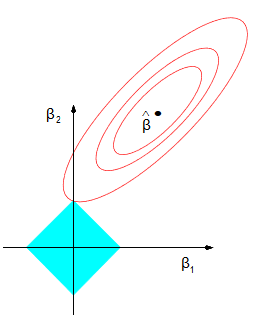
\includegraphics[width=0.5\linewidth]{Credit_Images/Lasso-regression.png}
   \caption{Boundary of lasso model.\cite{Hastie2009ThePrediction}}
    \label{fig-lasso}
\end{figure}

\subsubsection{Selecting the regularization coefficient}
As discussed in the previous Section the higher we set the value of the regularization term the stricter we constrain the weight coefficients. Therefore the larger $\lambda$ is the stricter the feature selection is as more coefficients will be set to 0. In order to select a $\lambda$ that provides us with the best features we need to tune this as a hyper parameter by using our validation set. We need to make sure that we do not throw away any features that have information that cannot be explained by the selected features. Therefore we tune $\lambda$ by making it stricter and monitoring how it affects the performance of the model. In Figure \ref{fig-regularizer} we have plotted the results of the \emph{accuracy}, \emph{recall}, and \emph{precision} metrics against a stronger penalty. Note that the L1 coefficient in this case is inversely proportional to how strict the regularizer is. As we can see both the recall and precision takes quite a significant drop once $\lambda$ reaches $0.0001$. Therefore $0.001$ is the smallest that we can set $\lambda$ before we start noticing a drop in the performance of the model. Setting $\lambda$ to $0.001$ reduces the number of features from 33 to 17. This is a big reduction while hardly losing any strength within the model, this may not be the most stable approach if we are looking to productionize this model but it allows the interpretation to be simpler to showcase due to the reduced number of attributions. These features are described in Chapter \ref{sect-Feature-Descriptions}.
\begin  {figure}[!htpb]
\centering
  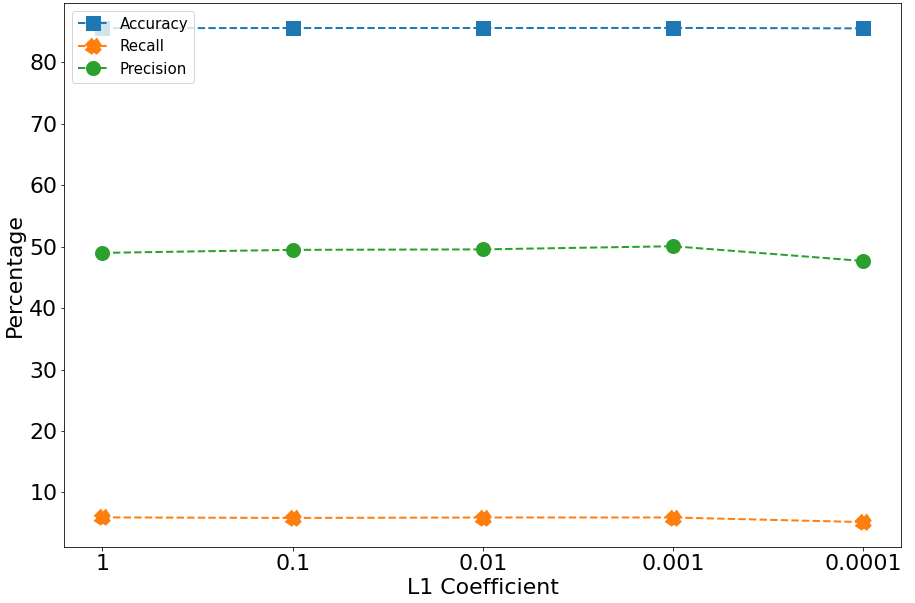
\includegraphics[width=\linewidth]{Credit_Images/Regularizer.png}
   \caption{Choosing the L1 coefficient.}
    \label{fig-regularizer}
\end{figure}

\subsection{Class imbalance} \label{sec-class-imbalance}
Class imbalance has a significant effect on conventional classification techniques because they assume a balance of classes \cite{articled}. In credit companies it is expected that there is a noticeable class imbalance within their data because they can not afford to have many bad loans \cite{809773}\cite{doi:10.1142/9789812813312_0009}. This results in there being far more loans which could be considered \emph{good}. This makes it difficult for many machine-learning techniques to learn the boundary between a good and bad loan because it does not have enough bad loans to properly identify them. Selectively sampling from the data in order to create a balanced dataset \cite{article} is a possible solution however this results in a far smaller training set and thus has an overall negative impact if we have a small sample size. It can be shown that by providing misclassification costs to our model provides an increase in the performance of classifiers  \cite{Vinciotti2003ScorecardCW}.  If we suppose that misclassifying a client that belongs to the \emph{default} as the \emph{not default} class is $r$ times as serious as the reverse. We can provide a weighting which penalize such misclassifications $r$ times as heavily as the reverse. In order to minimise the overall weighted misclassification rate we have to minimise,
\begin{equation}
  \mbox{ Assign to class} \ 1 \ \mbox{if} \ p(1|x) > (1 + r)^{-1} \mbox{and to class} \ 0 \ \mbox{otherwise}
\end{equation}
  We can incorporate these misclassification costs into our model by providing a weighting of classes which penalizes the model more for predicting the less present class incorrectly which is the \emph{default} class in our case. By using these bias class weights we may be able to identify more clients which may default, however we lose some accuracy in predicting non-defaulting clients. 
\begin{equation}
    \mbox{Class weights} = \frac{|X|}{|y| \cdot \left[ y_{1}, ..., y_{n} \right]}
\end{equation}
Where $|X|$ is the number of samples, $|y|$ is the number of classes, $y_{i}$ is the number of labels of class $i$.
By using the values in our dataset we get,
\begin{flalign}
    \begin{split}
    \mbox{Class weights} &= \frac{120000}{2 \cdot \left[102739, 17261 \right]}
    \\
                         &= [0.584, 3.476]
    \end{split}
\end{flalign}
by using these class weights the model is penalized roughly $5.95$ times more for incorrectly classifying \emph{defaulting} clients as \emph{not defaulted}. This causes the weights to be optimized to predict the default class more. For the raw input models we will use versions with and without these biased class weights and compare their results and how their interpretations differ.

\section{Models}
\subsection{Logistic Regression}
Logistic Regression is a widely used technique. Even some Deep Neural Networks use it within their output layer. It is known to work well for binary classification problems and provides a soft prediction. 
\subsubsection{Soft Predictions}
A soft prediction refers to a prediction which gives the probability that a input belongs to a specific class, where as a hard prediction simply assigns a 0 or 1 regardless if the prediction was on the boundary between the two classes. In Figure \ref{fig:thresholds} we can see the difference between the thresholding mechanisms used in hard and soft predictions, the x-axis represents the output before  we threshold and the y-axis is the value that after it goes through the activation function. When using a hard threshold the values are either set to 0 or 1. For soft threshold the value is set as a probability between 0 and 1, this allows us to see the confidence of the model in the prediction. For example in Figure \ref{fig:thresholds} if the value is 0, hard thresholding will force it to 1, however soft thresholding would set it to 0.5 which indicates that it could belong to either class. 

\subsubsection{Making a prediction using Logistic Regression}
Given a general linear model,
\begin{equation}
    y = \sum^{n}_{i = 1} w_{i} \cdot x_{i} + w_{0},
    \label{eq:linear}
\end{equation}
where $n$ is the number of features in the input.
We introduce the logistic function, or more commonly referred to as \emph{sigmoid}\cite{10.5555/1671238},
\begin{equation}
    \mbox{Sigmoid}(z) = \frac{1}{1 + e^{-z}}
\end{equation}
Substituting in (\ref{eq:linear}), this can be rewritten as,
\begin{equation}
    \mbox{Sigmoid}(w \cdot x + w_{0}) = \frac{1}{1 + e^{-(w \cdot x + w_{0})}}
    \label{eq:logistic}
\end{equation}
Once the model is trained, we substitute the input vector into (\ref{eq:logistic}) in order to make a prediction.
\begin{figure}
\centering
\begin{subfigure}{.5\textwidth}
  \centering
  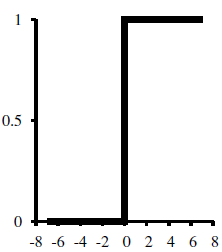
\includegraphics[width=\linewidth]{Credit_Images/hard_threshold.png}
  \caption{Hard Threshold}
  \label{fig:hard-threshold}
\end{subfigure}%
\begin{subfigure}{.5\textwidth}
  \centering
  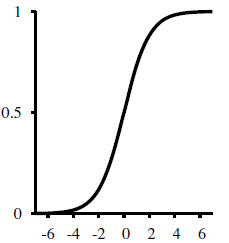
\includegraphics[width=\linewidth]{Credit_Images/soft_threshold.png}
  \caption{Soft Threshold}
  \label{fig:soft-threshold}
\end{subfigure}
\caption{Comparison of hard and soft thresholds\cite{10.5555/1671238}.}
\label{fig:thresholds}
\end{figure}
\subsubsection{Cross entropy cost function}
The cost function can be seen as a measurement of how incorrect the model is at estimating the relationship between the input $X$ and their corresponding labels $y$. It can also be seen as the distance between the predicted labels and the actual labels.
Let the sigmoid function of the model be $h_{w}(x)$ and the cost function be $J(w)$ then,
\abovedisplayskip=0pt\relax
\[
J(w) =
\begin{cases}
-\log(h_{w}(x)) & \text{if } y=1\\
-\log(1 - h_{w}(x)) & \text{if } y=0
\end{cases}
\]
can be condensed as,
\begin{equation}
J(w) = - \frac{1}{m} \sum_{i=1}^{m} \left[ y^{(i)}log(h_{w}(x^{(i)})) + (1 - y^{(i)})log(1-h_{w}(x^{(i)}))\right]
\end{equation}
Now that we have the cost function, we need to somehow decrease it until the weights converge.

\subsubsection{Gradient Descent}
In order to find the optimal parameters for the weights we have to minimize the cost function using gradient descent. Let $y$ be the true labels and $h_{w}(x)$ be the predicted labels. When using gradient descent, we set the weights to some initial value either randomly or by some initialization algorithm. We can update the weights by subtracting the derivative of the cost function,

\begin{equation}
w_{j} \longleftarrow w_{j} - \alpha \cdot \nabla_{w}J(w)
\end{equation}
where $\alpha$ is referred to as the \emph{learning rate} which is how large the steps we take when updating the weights are. Since $h_{w}$ is the sigmoid function we can simplify this to, 
\begin{equation}
    w_{j} \longleftarrow w_{j} - \alpha \sum_{i=1}^{m}(h_{w}(x^{(i)}) - y^{(i)})x_{j}^{(i)}
\end{equation}
This continues until the weights have converged.
In Figure \ref{fig-gradient-descent} we can see how the weights update during gradient descent. We start at some initial weights and after each weight update iteration we try to reach the minimum of the cost function. When we reach the minimum, the weights are considered to have converged and the training is completed as we have found the optimal parameters. Note that most if not all of the popular optimization procedures in Neural Networks is based on this simple idea, because the gradient can be efficiently calculated using \emph{back-propagation}. It should also be noted that numerous important modifications have been made for the sake of efficiency and robustness.
\begin {figure}[!htpb]
\centering
  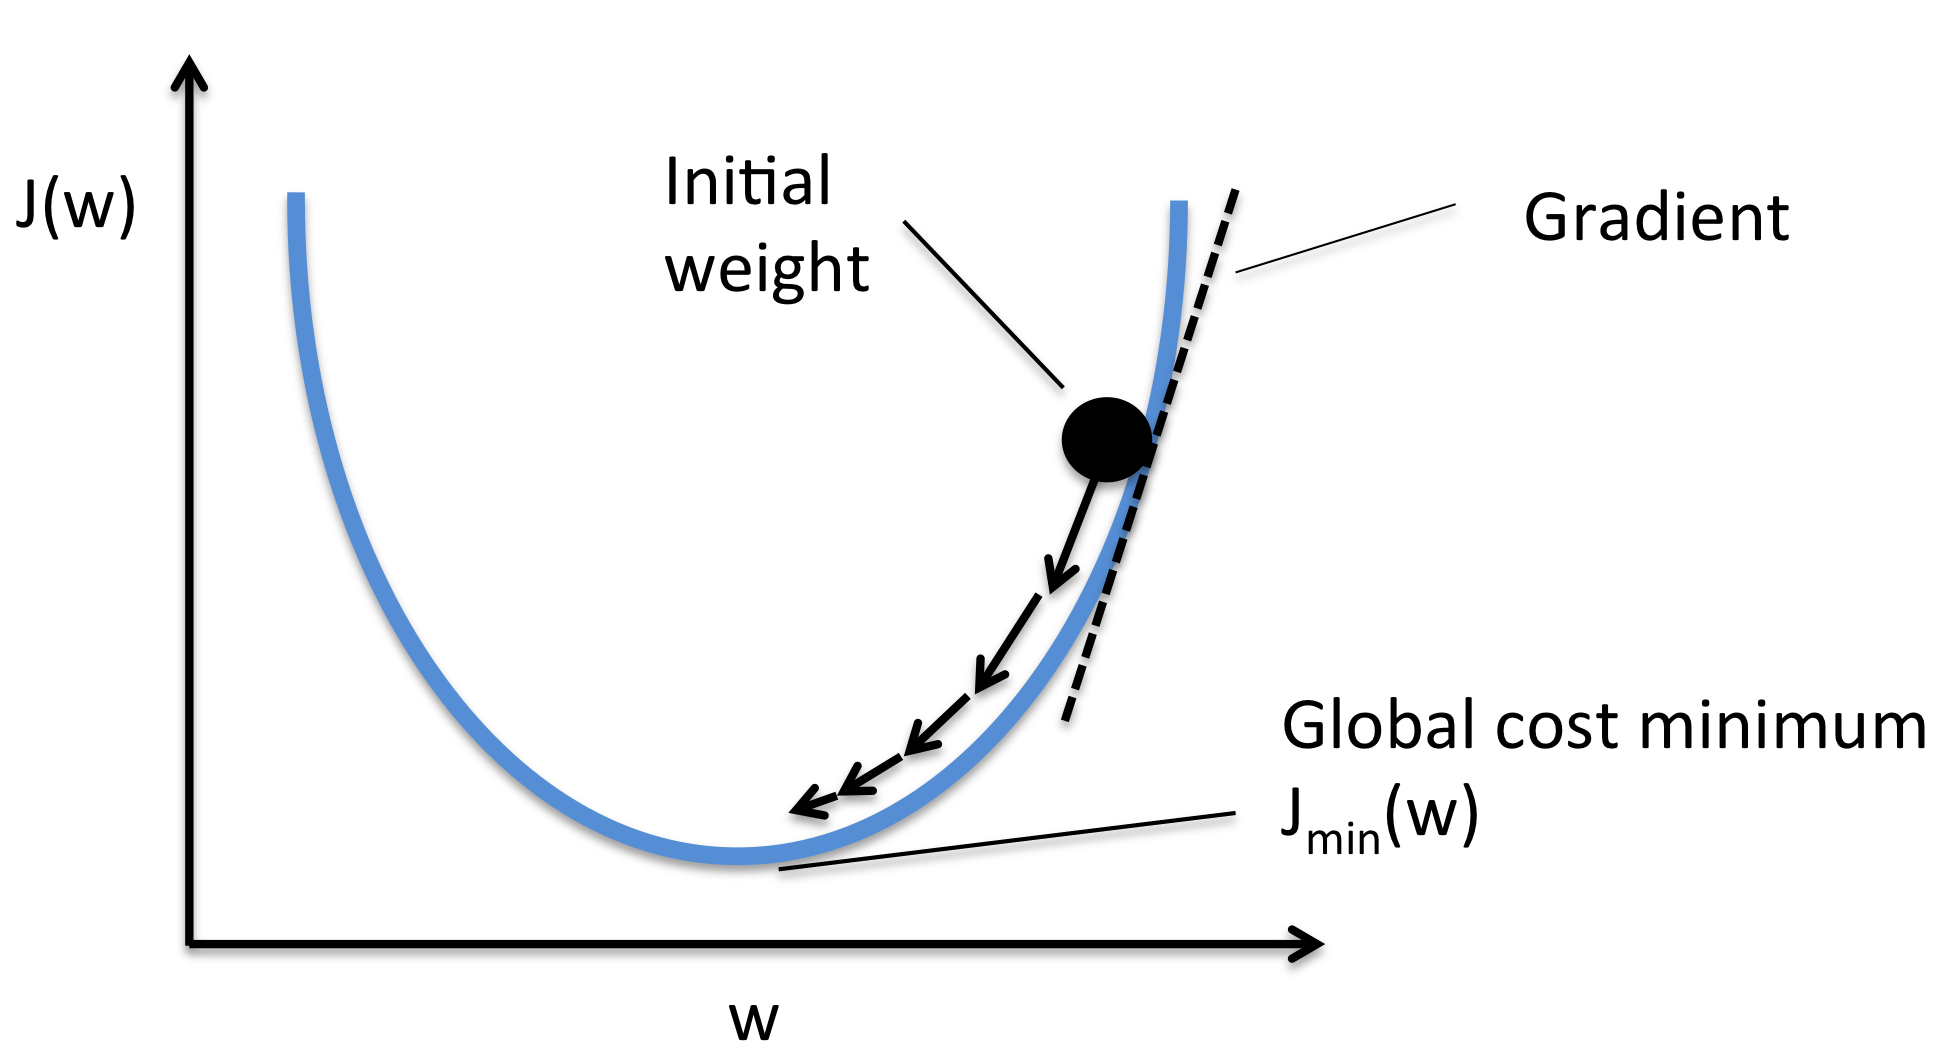
\includegraphics[width=\linewidth]{Credit_Images/GradientDescent.png}
   \caption{Gradient Descent \cite{GradientDescent}}
    \label{fig-gradient-descent}
\end{figure}

\subsubsection{Interpreting Logistic Regression} \label{sect:interpreting-logistic-regression}
Since the outcome of Logistic Regression is a probability between 0 and 1, we can not simply look at the weight coefficients as a direct interpretation. The weighted sum in the linear equation (\ref{eq:linear}) is transformed into a probability by the sigmoid function (\ref{eq:logistic}). Therefore the weights do not affect the probability linearly. Introducing the log odds function,

\begin{equation}
    \log \left( \frac{P(y=1)}{1 - P(y=1)} \right) = \log \left( \frac{P(y=1)}{P(y=0)} \right) = w_{0} + w_{1}x_{1} + ... + w_{n}x_{n}
\end{equation}
We can adjust this equation in order to determine how the prediction changes when one feature $x_{j}$ is changed by 1 unit \cite{molnar2019}. Applying the exp function to both sides we end up with,

\begin{equation}
     \frac{P(y=1)}{1 - P(y=1)} = odds = \exp( w_{0} + w_{1}x_{1} + ... + w_{n}x_{n})
\end{equation}
Comparing the ratio of two predictions when increasing a single feature by 1,

\begin{equation}
    \frac{odds_{x_{j}+1}}{odds} = \frac{\exp^( w_{0} + w_{1}x_{1} + ... + w_{j}(x_{j} + 1) + ... w_{n}x_{n})}{exp^( w_{0} + w_{1}x_{1} + ... + w_{j}x_{j} + ... w_{n}x_{n})}
\end{equation}
Then applying the following exponential rule,

\begin{equation}
    \frac{\exp(a)}{\exp(b)} = \exp(a - b)
\end{equation}
and removing many terms,

\begin{equation}
    \frac{odds_{x_{j}+1}}{odds} = \exp(w_{j}(x_{j} + 1) - w_{j}x_{j}) = \exp(w_{j})
    \label{eq-odds-ratio}
\end{equation}
The \emph{Odds Ratio (OR)} can be seen as a measurement of the strength between 2 events. Given 2 events $A$ and $B$, we can define the OR as the ratio of the odds of A occurring in the presence of B compared to the odds of A occurring in the absence of B \cite {Szumilas2010ExplainingRatios}.
\begin{itemize}
    \item OR=$1$ The events $A$ and $B$ are independent.
    \item OR$>1$ If $B$ is present then A has higher odds of occurring .
    \item OR$<1$ If $B$ is absent then $A$ has higher odds of occurring.
\end{itemize}
Therefore according to (\ref{eq-odds-ratio}) a change in a feature by one unit changes the odds ratio (multiplicative) by a factor of $\exp(w_{j})$. Another interpretation is that by changing a feature's value by one unit increases the log odds ratio by the value of the corresponding weight \cite{molnar2019}. Interpretation is different depending on the feature type \cite{molnar2019}:
\begin{itemize}
    \item \emph{Numerical features}: If you increase the value of feature $x_{j}$ by one unit, the estimated odds change by a factor of $\exp(w_{j})$
    \item \emph{Binary categorical features}: We refer to one of the categories as the \emph{reference} category. Changing the feature $x_{j}$ from the reference category to the other category in turn changes the estimated odds by a factor of $\exp(w_{j}))$.
    \item \emph{Categorical feature with more than two categories}:  When dealing with multiple categories one-hot-encoding is commonly used. For a feature which has N categories we would need N-1 columns in our one-hot-encoder. The N-th category is  considered the reference category. The interpretation for each category then is equivalent to the interpretation of binary features.
\end{itemize}
In table \ref{table:logistic} we can see an example of a Logistic Regression classifier trained to predict the probability of cervical cancer given certain risk factors  \cite{molnar2019}. Looking at the \emph{Num. of diagnosed STDs} feature which is numerical, increasing the number of STDs by 1 would in turn increase the odds of cancer vs. no Cancer by a factor of 2.26. Looking at the feature \emph{Hormonal contraceptives y/n} which is a binary categorical feature indicates that for women who use hormonal contraceptives, the odds for cancer vs. no cancer are by a factor of 0.89 lower, compared to women without hormonal contraceptive. It is important to note that these interpretations are only true if every other feature stays the same.
 \begin{table}[h!]
 \footnotesize
\begin{center}
\shadowbox{\begin{minipage}[t]{0.75\columnwidth}%
    \begin{tabular}{l|c|c|c}
         & \textbf{Weight} & \textbf{Odds ratio} & \textbf{Std. Error}\\
            \hline
         Intercept & $-2.91$ & $0.05$ & $0.32$ \\
         Hormonal contraceptives y/n & $-0.12$ & $0.89$ & $0.30$ \\
         Smokes y/n & $\phantom{-}0.26$ & $1.29$ & $0.37$ \\
         Num. of pregnancies & $\phantom{-}0.04$ & $1.04$ & $0.10$ \\
         Num. of diagnosed STDs & $\phantom{-}0.82$ & $2.26$ & $0.33$ \\
         Intrauterine device y/n & $\phantom{-}0.62$ & $1.85$ & $0.40$ \\
    \end{tabular}
    \end{minipage}}
\par\end{center}
\caption{The results of fitting a logistic regression model on the cervical cancer dataset. Shown are the features used in the model, their estimated weights and corresponding odds ratios, and the standard errors of the estimated weights. \cite{molnar2019}}\label{table:logistic}
\end{table}

\subsection{Feedforward Neural Network}
We will be training a generic feedforward Neural Network with a single hidden layer. The architecture can be seen in Figure \ref{fig-ff-nn}. Every layer in the Neural Network is \emph{Fully Connected} which means that every incoming node is connected to every outgoing node. The input layer is simply the input features. The \emph{hidden layer} contains $9$ nodes for the raw features and $11$ nodes for the WOE network. For both networks the output layer is a single node that uses the \emph{sigmoid} activation function which is the probability that the client will default. The Neural Network only has a single hidden layer and is considered very small when compared to modern networks.

\begin  {figure}[!htpb]
\centering
  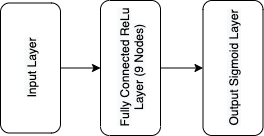
\includegraphics[width=0.5\linewidth]{Credit_Images/Credit_Architecture.png}
   \caption{Architecture of credit Neural Network.}
    \label{fig:weight-tab}
\end{figure}

\subsection{Trainable weights}
In order to show that a Neural Network is theoretically more powerful than Logistic Regression, we have to compare their \emph{trainable weights}. Trainable weights are the weights which models will estimate in order to make a prediction. Theoretically the more weights we can estimate, the more accurate the predictions will be. However it is important that we account for \emph{overfitting} which is when the model corresponds too closely to the training data and thus fails to predict unseen data reliably. In practice there are other factors such as the networks architecture and preprocessing techniques which have an effect. We can calculate the trainable weights with,

\begin{equation*}
\begin{split}
    \mbox{LR} &= \mbox{Input weights} + \mbox{Intercept}
    \\
    \mbox{NN} &= \mbox{Input weights} \cdot \mbox{Hidden weights} + \mbox{Hidden weights} \cdot \mbox{Output weights}
    \end{split}
\end{equation*}
We can see the comparison of the trainable weights between the models in Figure \ref{table:trainable}.
 \begin{table}[h!]
 \footnotesize
\begin{center}
\shadowbox{\begin{minipage}[t]{\columnwidth}%
    \begin{tabular}{lccccc}
       \textbf{Model}  & \textbf{Input} & \textbf{Hidden} & \textbf{Output} & \textbf{Intercept} & \textbf{Trainable Weights}\\
        Logistic Regression & $17$ & 0 & 1 & $\checkmark$ &  18\\
        Logistic Regression WOE & $22$ & 0 & 1 & $\checkmark$ & 23\\
        Neural Network & $17$ & 9 & 1 & $\times$ & 162\\
        Neural Network WOE & $22$ & 11 & 1 & $\times$ & 253\\
    \end{tabular}
    \end{minipage}}
\par\end{center}
\caption{Trainable Weights}\label{table:trainable}
\end{table}
%%%% RESULTS %%%%
\section{Results}
In this Chapter we will compare the following models:
\begin{itemize}
    \item Logistic Regression with raw inputs.
    \item Logistic regression with raw inputs and altered class weights.
    \item Logistic Regression with WOE inputs.
    \item Neural Network with raw inputs.
    \item Neural Network with raw inputs and altered class weights.
    \item Neural Network with WOE inputs.
\end{itemize}

\begin {figure}[!htpb]
\centering
  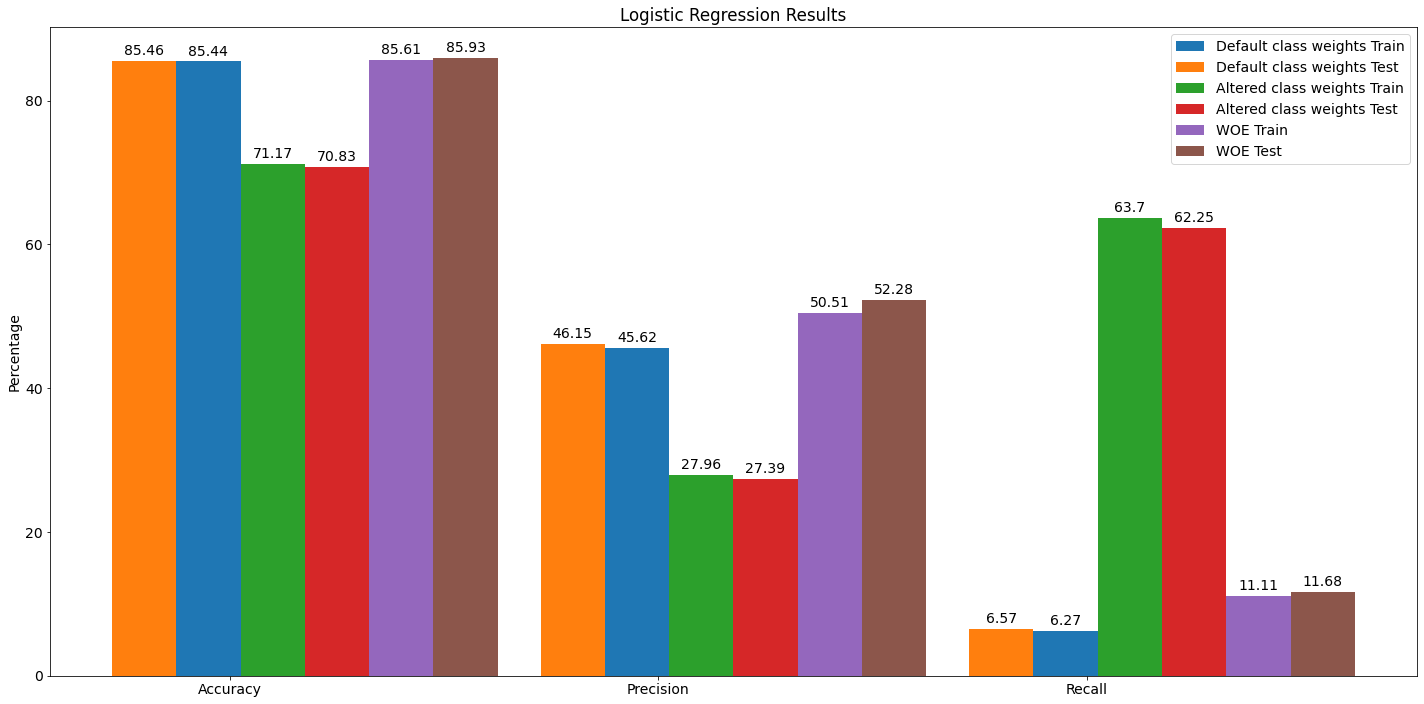
\includegraphics[width=\linewidth]{Credit_Images/Results_Logistic.png}
   \caption{Results of the Logistic Regression classifier.}
    \label{fig-log-results}
\end{figure}
\begin {figure}[!htpb]
\centering
  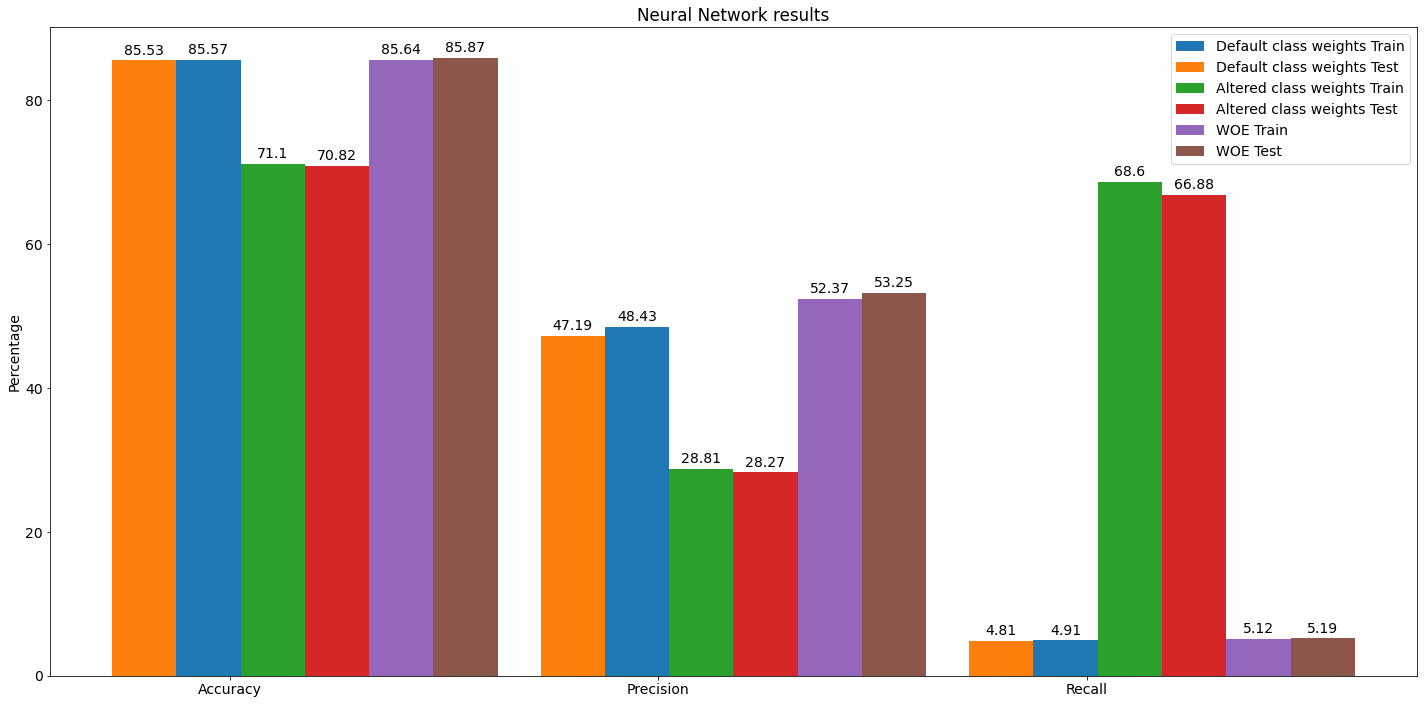
\includegraphics[width=\linewidth]{Credit_Images/NN_res.png}
   \caption{Results of the Neural Network.}
    \label{fig-nn-results}
\end{figure}

\subsection{Comparison}
Comparing the results from the Logistic Regression classifier in Figure \ref{fig-log-results} and Neural Network classifier in Figure \ref{fig-nn-results} their \emph{accuracy} is mostly the same with the only real difference being a slight increase in \emph{precision} and \emph{recall} in the Neural Network. From this it may seem that there is no reason to use a Neural Network classifier, however there are plenty of optimizations and various other network compositions that may provide better results. Our purpose is to provide interpretability and therefore we are not concerned with building the most robust network possible.
\subsection{Normal vs Bias class weights}
In both models when using the bias class weights discussed in Chapter \ref{sec-class-imbalance} we see on average a $15\%$ drop in accuracy which is quite significant, however an enormous increase in \emph{recall} which means the bias versions are better at identifying clients which \emph{defaulted}. For credit companies where the purpose is to identify clients which may default on their loans, the bias weights provide better results. In the upcoming \emph{Interpretation} Section we compare both the normal and bias class weights models and observe the explanations produced by SHAP in order to compare the difference in feature attributions. 
\subsection{Raw Inputs vs WOE}
When looking at the comparisons from the raw input features to the WOE transformed features in both the Logistic Regression results in Figure \ref{fig-log-results} and the Neural Network results in Figure \ref{fig-nn-results} there does not some to be a significant difference. The only noticeable difference is a slight increase in precision. WOE transformation are the standard when working in the credit industry and from these results it may seem like there isn't much merit in it, but we will see in the \emph{explanations} in Section \ref{sec-interpretation} that there is a significant difference.
 \section{Feature descriptions} \label{sect-Feature-Descriptions}
 In order to make sense of the feature attributions we first have to describe what each feature means. From our credit domain knowledge we are able to specify which features magnitudes increase proportionally to the risk that the client will default.
 
 \subsection{Not Default}
 The following features decrease the risk of the client defaulting,
 \begin{description}
     \item[age (For clients who are middle-aged)] \hfill \\ The age of the client.
     \item[regular\_income\_flg] \hfill \\ A flag which indicates whether the client has a regular income or not.
     \item[tot\_available\_limit] \hfill \\ Total monthly limit available to client.
 \end{description}
 \subsection{Default}
 The following features increase the risk of the client defaulting,
 \begin{description}
     \item[age (For clients who are very young or old)] \hfill \\ The age of the client.
     \item[requested\_amt\_l1m] \hfill \\ Requested amount over a month.
     \item[requested\_amt\_l24m] \hfill \\ Requested amount over 24 months.
     \item[requested\_amt\_to\_income] \hfill \\ Ratio of requested amount to monthly income.
     \item[avg\_credit\_cost] \hfill \\ Average cost of credit.
     \item[avg\_remaining\_loan\_term] \hfill \\ The average amount of months left on the clients loans.
     \item[tot\_monthly\_instalment] \hfill \\ Monthly installment paid towards the loan.
     \item[monthly\_inst\_to\_income] \hfill \\ Ratio of income to monthly installment.
     \item[tot\_credit\_searches\_l1m] \hfill \\ Total credit searches in the last month.
     \item[tot\_credit\_searches\_l3m] \hfill \\ Total credit searches in the last 3 months.
     \item[tot\_credit\_searches\_l6m] \hfill \\ Total credit searches in the last 6 months.
     \item[tot\_credit\_searches\_l12m] \hfill \\ Total credit searches in the last 12 months.
     \item[tot\_credit\_searches\_l24m] \hfill \\ Total credit searches in the last 24 months.
     \item[worst\_status\_flg] \hfill \\ Flag of whether this loan is the most in arrears.
     \item[tot\_declines\_l12m] \hfill \\ Total credit declines in the last 12 months.
     \item[active\_loans\_in\_arrears] \hfill \\ Active loans that are in arrears.
     \item[tot\_loans\_in\_arrears] \hfill \\ Total loans that are in arrears.
     \item[worst\_arrears\_l1m] \hfill \\ Worst arrears in the past month.
     \item[worst\_arrears\_l3m] \hfill \\ Worst arrears in the past 3 months.
     \item[worst\_arrears\_l6m] \hfill \\ Worst arrears in the past 6 months.
     \item[worst\_arrears\_l12m] \hfill \\ Worst arrears in the past 12 months.
     \item[worst\_arrears\_l24m] \hfill \\ Worst arrears in the past 24 months.
     \item[tot\_balance\_due] \hfill \\ Total balance due on the loan.
 \end{description}
%%%% Interpretation %%%%
\section{Interpretation} \label{sec-interpretation}
In this Section we observe how the inherent interpretability of Logistic Regression compares to the explanations provided by SHAP of the Neural Network. We provide interpretation for both the normal and bias class weights models as well as a comparison between the attributions generated by the WOE features compared to the raw features.
\subsection{Logistic Regression}
As we have discussed in Section \ref{sect:interpreting-logistic-regression} for Logistic Regression the weight coefficients are not enough to provide interpretability.  We have to extract the weight coefficients $w$ from the linear equation (\ref{eq:linear}) and also calculate their odds ratio (which is described in Section \ref{sect:interpreting-logistic-regression}) with (\ref{eq-odds-ratio}). We have tabulated the weight coefficients as well as their respective odds ratios. We have also graphed the odds ratio for extra clarity. Table \ref{table:logistic} and Figure \ref{fig-odds-lr}  is for the raw input model. Table \ref{table:logistic-weighted} and Figure \ref{fig-odds-weighted} is for the raw input model with altered class weights. Lastly Table \ref{table:logistic-woe} and Figure \ref{fig-odds-woe} is for the WOE model.

\subsubsection{WOE weight coefficients}
From Table \ref{table:logistic-woe} we can see that all of the weight coefficients are positive for the WOE classifier. It may seem like every variable positively contributes towards the \emph{default} class. This is however not the case as we do not know the range of the magnitudes of the variables by just looking at this table. If the woe value of a feature in a specific bin is negative then even if the weight coefficient is positive it will provide a negative attribution. Therefore Table \ref{table:logistic-woe} can not be considered sufficient information as we would need to view the range of the feature values to discern whether a feature decreases or increases the probability of \emph{defaulting}.

 \begin{table}[h!]
 \footnotesize
\begin{center}
\shadowbox{\begin{minipage}[t]{0.55\columnwidth}%
    \begin{tabular}{l|c|c}
         \textbf{Feature} & \textbf{Weight} & \textbf{Odds ratio}\\
            \hline
         requested\_amt\_l24m & $\phantom{-}0.0028$ & $1.002804$ \\
         tot\_declines\_l12m & $\phantom{-}0.0098$ & $1.009848$ \\
         requested\_amt\_to\_income & $\phantom{-}0.0109$ & $1.010960$  \\
         tot\_credit\_searches\_l12m & $-0.0207$ & $0.979513$  \\
         worst\_arrears\_l24m & $\phantom{-}0.0233$ & $1.023574$  \\
         tot\_available\_limit & $-0.0305$ & $0.969960$  \\
         tot\_credit\_searches\_l3m & $\phantom{-}0.0335$ & $1.034067$  \\
         age & $-0.0474$ & $0.953706$ \\
         tot\_loans\_in\_arrears & $\phantom{-}0.0565$ & $1.058127$ \\
         regular\_income\_flg & $-0.0645$ & $0.937536$ \\
         tot\_monthly\_installment & $-0.0659$ & $0.936224$ \\
         worst\_status\_flg & $\phantom{-}0.0676$ & $1.069937$ \\
         avg\_credit\_cost & $\phantom{-}0.0781$ & $1.081231$  \\
         monthly\_inst\_to\_income & $\phantom{-}0.0832$ & $1.086759$  \\
         avg\_remaining\_loan\_term & $\phantom{-}0.0846$ & $1.088282$  \\
         worst\_arrears\_l6m & $\phantom{-}0.1027$ & $1.108159$  \\
         active\_loans\_in\_arrears & $-0.2181$ & $0.804045$  \\

    \end{tabular}
    \end{minipage}}
\par\end{center}
\caption{Weight coefficients for Logistic Regression}\label{table:logistic}
\end{table}

\begin  {figure}[!htpb]
\centering
  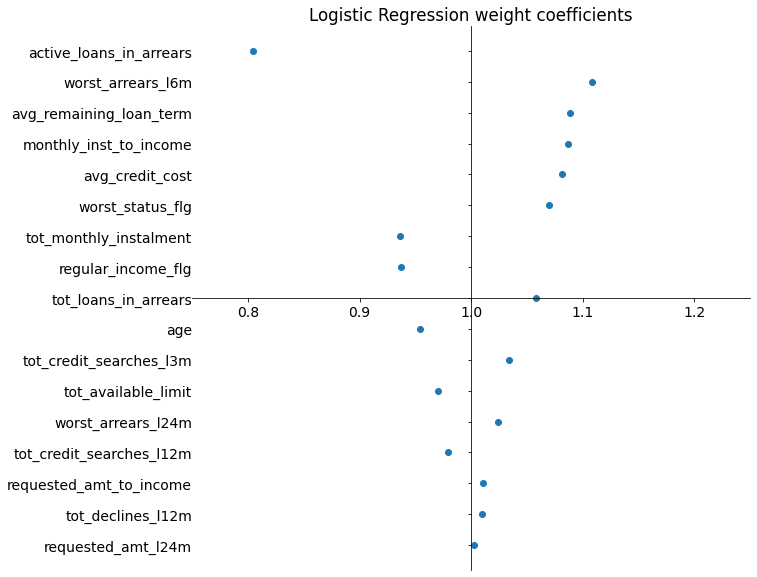
\includegraphics[width=0.8\linewidth]{Credit_Images/LR_ODDS.png}
   \caption{Odds ratios for Logistic Regression}
    \label{fig-odds-lr}
\end{figure}


 \begin{table}[h!]
 \footnotesize
\begin{center}
\shadowbox{\begin{minipage}[t]{0.55\columnwidth}%
    \begin{tabular}{l|c|c}
         \textbf{Feature} & \textbf{Weight} & \textbf{Odds ratio}\\
            \hline
         requested\_amt\_l24m & $-0.0076$ & $0.992429$  \\
         tot\_declines\_l12m & $\phantom{-}0.0497$ & $1.050956$ \\
         requested\_amt\_to\_income & $\phantom{-}0.0161$ & $1.016230$   \\
         tot\_credit\_searches\_l12m & $-0.0172$ & $0.982947$  \\
         worst\_arrears\_l24m & $\phantom{-}0.0769$ & $1.079934$   \\
         tot\_available\_limit &  $\phantom{-}0.0171$ & $1.017247$ \\
         tot\_credit\_searches\_l3m & $\phantom{-}0.0539$ & $1.055379$  \\
         age & $-0.0375$ & $0.963194$   \\
         tot\_loans\_in\_arrears & $\phantom{-}0.0339$ & $1.034481$  \\
         regular\_income\_flg & $-0.0481$ & $0.953038$ \\
         tot\_monthly\_installment & $-0.0819$ & $0.921364$ \\
         worst\_status\_flg & $\phantom{-}0.0475$ & $1.048646$  \\
         avg\_credit\_cost & $\phantom{-}0.0941$ & $1.098670$   \\
         monthly\_inst\_to\_income & $\phantom{-}0.0989$ & $1.103956$   \\
         avg\_remaining\_loan\_term & $\phantom{-}0.0609$ & $1.062793$   \\
         worst\_arrears\_l6m & $\phantom{-}0.0773$ & $1.080366$  \\
         active\_loans\_in\_arrears & $-0.1814$ & $0.834102$  \\

    \end{tabular}
    \end{minipage}}
\par\end{center}
\caption{Weight coefficients for Logistic Regression with altered class weights.}\label{table:logistic-weighted}
\end{table}

\begin  {figure}[!htpb]
\centering
  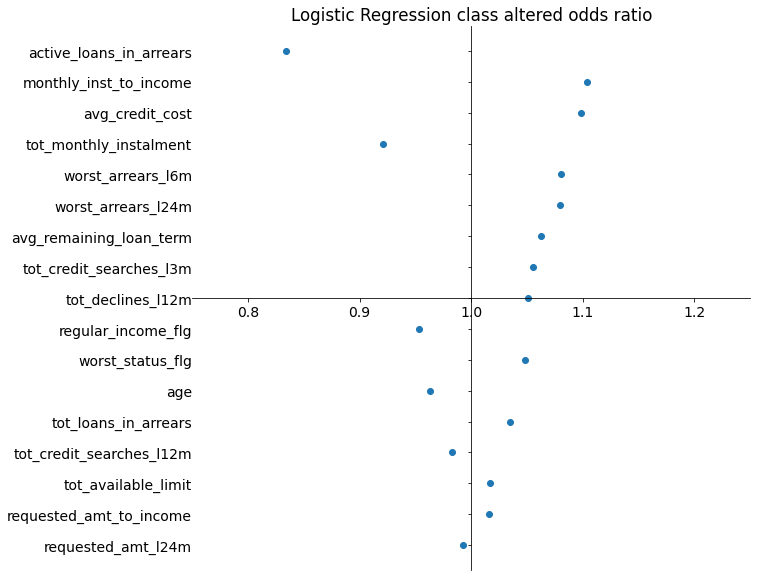
\includegraphics[width=0.8\linewidth]{Credit_Images/LR__ALTERED_ODDS.png}
   \caption{Odds ratios for Logistic Regression with altered class weights.}
    \label{fig-odds-weighted}
\end{figure}




 \begin{table}[h!]
 \footnotesize
\begin{center}
\shadowbox{\begin{minipage}[t]{0.6\columnwidth}%
    \begin{tabular}{l|c|c}
         \textbf{Feature} & \textbf{Weight} & \textbf{Odds ratio}\\
            \hline
            tot\_monthly\_instalment\_woe & $1.001401$ & $0.0014$ \\
            worst\_arrears\_l1m\_woe & $1.002102$ & $0.0021$ \\
            tot\_credit\_searches\_l6m\_woe & $1.004108$ & $0.0041$ \\
            worst\_arrears\_l3m\_woe & $1.009041$ & $0.0090$ \\
            worst\_status\_flg\_woe & $1.010859$ & $0.0108$ \\
            worst\_arrears\_l12m\_woe & $1.012984$ & $0.0129$ \\
            tot\_credit\_searches\_l24m\_woe & $1.015621$ & $0.0155$ \\
            tot\_credit\_searches\_l12m\_woe & $1.016332$ & $0.0162$ \\
            tot\_credit\_searches\_l1m\_woe & $1.017145$ & $0.0170$ \\
            requested\_amt\_to\_income\_woe & $1.024188$ & $0.0239$ \\
            worst\_arrears\_l6m\_woe & $1.040603$ & $0.0398$ \\
            tot\_credit\_searches\_l3m\_woe & $1.053376$ & $0.0520$ \\
            monthly\_inst\_to\_income\_woe & $1.056541$ & $0.0550$ \\
            tot\_loans\_in\_arrears\_woe & $1.057280$ & $0.0557$ \\
            avg\_credit\_cost\_woe & $1.059079$ & $0.0574$ \\
            tot\_balance\_due\_woe & $1.061412$ & $0.0596$ \\
            tot\_available\_limit\_woe & $1.064814$ & $0.0628$ \\
            requested\_amt\_l1m\_woe & $1.067159$ & $0.0650$ \\
            worst\_arrears\_l24m\_woe & $1.078100$ & $0.0752$ \\
            avg\_remaining\_loan\_term\_woe & $1.102963$ & $0.0980$ \\ 
            active\_loans\_in\_arrears\_woe & $1.109268$ & $0.1037$ \\
            age\_woe & $1.176919$ & $0.1629$

    \end{tabular}
    \end{minipage}}
\par\end{center}
\caption{Weight coefficients for WOE Logistic Regression.}\label{table:logistic-woe}
\end{table}

\begin  {figure}[!htpb]
\centering
  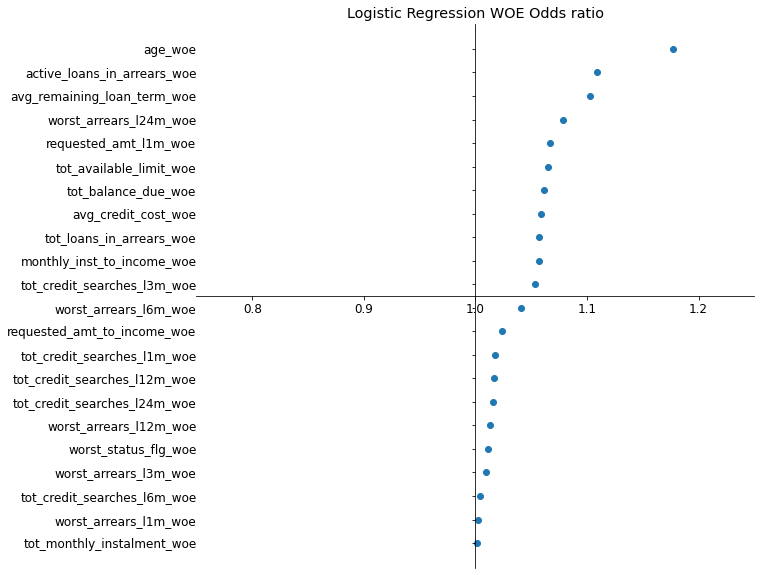
\includegraphics[width=0.8\linewidth]{Credit_Images/LR_WOE_ODDS.png}
   \caption{Odds ratios for WOE Logistic Regression.}
    \label{fig-odds-woe}
\end{figure}


\subsection{Neural Network}
For the Neural Network we will be using \emph{Deep SHAP} as it leverages the composition of Neural Networks to significantly increase the speed of SHAP.
We will be looking at how SHAP explains individual predictions as well as the explanation for the entire model.
\subsubsection{Model explanation}
We start by explaining on a global level the attributions the model assigns to each input feature and compare it to the Logistic Regression explanations. Figure~ \ref{fig-deep-shap-NN} is the explanation for the normal network, Figure \ref{fig-deep-shap-weighted-NN} is for the bias class weights network, and Figure \ref{fig-deep-shap-WOE-NN} is the WOE network. Rather than just giving a single value for attributions SHAP is able to plot over multiple instances in the dataset and showcase how each feature attributes to different instances. The y-axes are the feature names and the x-axes are their corresponding SHAP values, larger values impacts the model more. Positive values attribute towards the \emph{default} class and negative values to the \emph{not default} class. The hue of a point ranges from blue to red where the redder a point the larger the magnitude of that feature was in that particular instance.
\paragraph{Explanation}
Using the information from Section \ref{sect-Feature-Descriptions} we know that the larger the magnitude of the \emph{Age} feature the more it contributes against the client defaulting. In Figure \ref{fig-deep-shap-NN} and \ref{fig-deep-shap-weighted-NN} we can see that the larger the magnitude of age the SHAP value falls more into the negative region, this indicates that the older the client is, the less likely they are to \emph{default}. This coincides with our knowledge. On the inverse we know that the \emph{avg\_credit\_cost} feature contributes towards the client \emph{defaulting}, this is also shown in Figure \ref{fig-deep-shap-NN} and \ref{fig-deep-shap-weighted-NN} where the instances where the larger the magnitude of \emph{avg\_credit\_cost} is, the larger it's SHAP value is and thus the higher contribution it had towards predicting that the client would default.

\begin  {figure}[!htpb]
\centering
  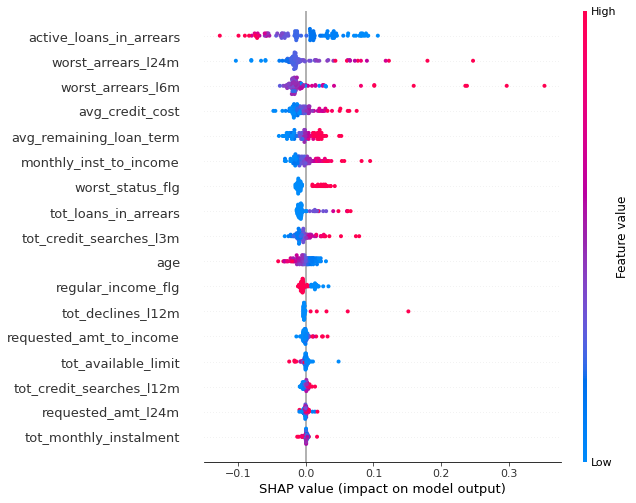
\includegraphics[width=0.8\linewidth]{Credit_Images/NN_shap_deep_summary.png}
   \caption{Deep SHAP interpretation for Neural Network.}
    \label{fig-deep-shap-NN}
\end{figure}

\begin  {figure}[!htpb]
\centering
  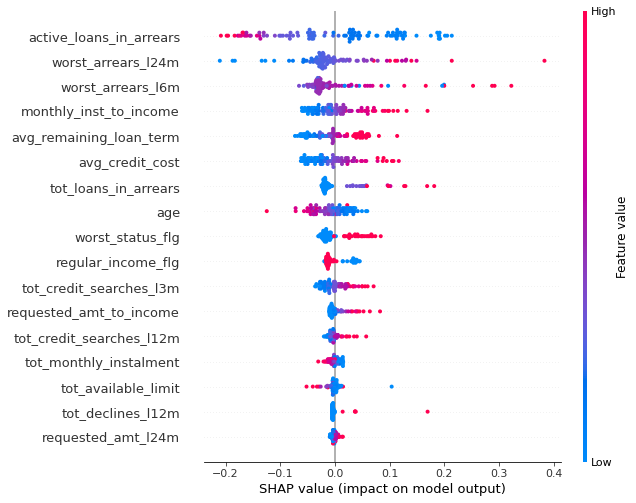
\includegraphics[width=0.8\linewidth]{Credit_Images/NN_shap_deep_weighted_summary.png}
   \caption{Deep SHAP interpretation for class weight bias Neural Network.}
    \label{fig-deep-shap-weighted-NN}
\end{figure}
\begin  {figure}[!htpb]
\centering
  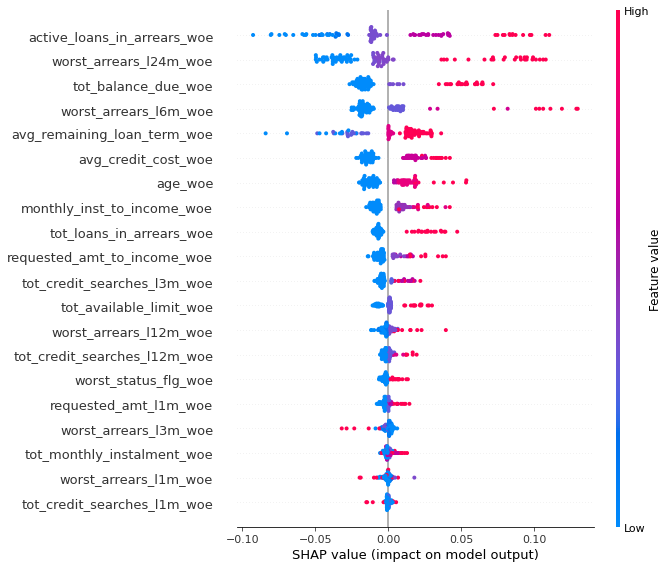
\includegraphics[width=0.8\linewidth]{Credit_Images/WOE_IV_NOSCALE_MODEL.png}
   \caption{Deep SHAP interpretation for WOE Neural Network.}
    \label{fig-deep-shap-WOE-NN}
\end{figure}

\subsubsection{Individual predictions}
An advantage of using a tool such as SHAP is that we are able to obtain explanations for individual predictions rather than just for the entire model. This is useful for credit employees as this allows them to obtain explanations for an individual client. We have chosen a single client which has \emph{defaulted} and in Figure \ref{fig-deep-shap-single-NN}, \ref{fig-deep-shap-weighted-single-NN} and \ref{fig-deep-shap-WOE-single-NN} we can see a plot of the explanation for it's prediction. Figure \ref{fig-deep-shap-single-NN} is the \emph{normal} class weights and the output of the model is that it is $27\%$ certain that the client will \emph{default on their loan}. Figure \ref{fig-deep-shap-weighted-single-NN} is the explanation for the \emph{bias} class weights model and it is $71\%$ certain that the client will \emph{default}. Figure \ref{fig-deep-shap-WOE-single-NN} is the explanation for the WOE Neural Network and it is $37\%$ that the client will \emph{default}. The y-axes are the input features and the x-axes is the model output value. The bottom of the line is the average model output value, which is the models default output value given that there is no information about the input features. As the line reaches the top, each feature either adds or subtracts from the models predicted value, therefore features that subtract from the value are negative attributions and those that add are positive attributions. The numbers in brackets are the values of that feature of this particular client standardized.

\begin  {figure}[!htpb]
\centering
  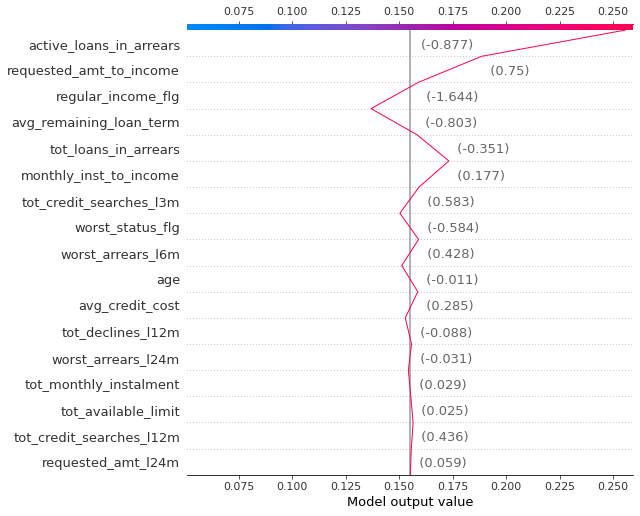
\includegraphics[width=0.8\linewidth]{Credit_Images/shap-nn-single.png}
   \caption{Single prediction Deep SHAP interpretation for Neural Network.}
    \label{fig-deep-shap-single-NN}
\end{figure}

\begin  {figure}[!htpb]
\centering
  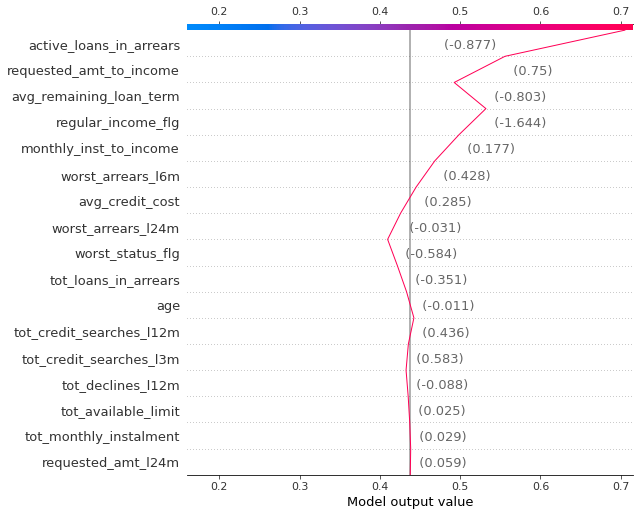
\includegraphics[width=0.8\linewidth]{Credit_Images/shap-nn-weighted-single.png}
   \caption{Single prediction Deep SHAP interpretation for class weight bias Neural Network.}
    \label{fig-deep-shap-weighted-single-NN}
\end{figure}

\begin  {figure}[!htpb]
\centering
  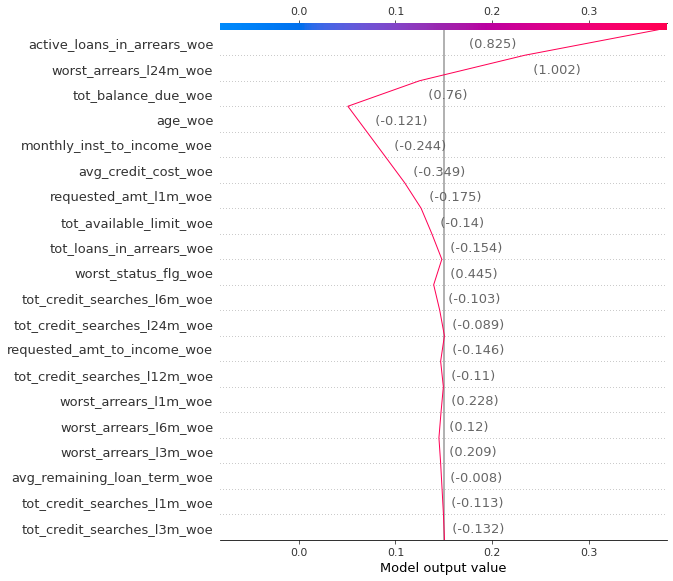
\includegraphics[width=0.8\linewidth]{Credit_Images/WOE_IV_NOSCALE_INDV.png}
   \caption{Single prediction Deep SHAP interpretation for WOE Neural Network.}
    \label{fig-deep-shap-WOE-single-NN}
\end{figure}


\subsection{Comparison} Comparing the weight coefficients obtained from Logistic Regression with the SHAP explanations we can see that although the SHAP values have a different meaning than the raw weight coefficients they are comparable. They both provide a relative value of how much that particular feature would affect the prediction of the model. The SHAP explanations are far more descriptive as they are able to provide explanations over multiple instances, which shows consistency and we are also able to provide explanations for individual instances. Since the SHAP values are consistent with what we expect we can conclude that we have successfully provided explanations into this previously considered \emph{black-box} credit risk Neural Network.

\subsection{Exposing a problem with the raw input models} \label{sect-problem-expose}
If we refer back to Section \ref{sect-Feature-Descriptions} we can see that  the \emph{active\_loans\_in\_arrears} feature is the number of active loans that the client currently has in arrears. An increase in its feature value would in turn cause the risk of the client to increase. As we can see for the WOE model in Figure \ref{fig-deep-shap-WOE-NN} the larger the magnitude of \emph{active\_loans\_in\_arrears} the higher the contribution towards the \emph{Default} class as expected. However looking at the SHAP explanations for the raw input models in Figure \ref{fig-deep-shap-NN} and \ref{fig-deep-shap-weighted-NN} the larger  \emph{active\_loans\_in\_arrears} is the less likely the client is to \emph{default} . This means that there is an obvious flaw present with the raw input models with regards to this feature. This is not obvious from just observing the Logistic Regression models since it hard to determine how the feature reacts over multiple instances and different magnitudes by only looking at the features overall contribution. Even though the performance of the two models are relatively the same by viewing the SHAP explanations produced, we were able to identify this problem.

\subsection{Monitoring changes within the architecture} \label{sect-architecure}
Figure \ref{fig-deep-shap-WOE-sig} is the SHAP explanation of the WOE Neural Network with the hidden layer removed form the network itself. When comparing this to Figure \ref{fig-deep-shap-WOE-NN} there is a noticeable difference as the \emph{worst\_arrears\_l24m\_woe} has the largest contribution. The explanation is expected to change but SHAP can provide some insight to what the changes are. When training a neural network one of the hardest problems is figuring out what the architecture should be. An example would be for a simple neural network how do we decide how many hidden layers? What about how many neurons in each layer? Usually we would just use our metrics and experiment with the architecture. However metrics don't really tell the whole story and with SHAP we can observe how the architecture affects the variables attributions themselves. Thus by using SHAP we are able to determine how a change in the networks architecture affects the feature attributions. 
\begin{figure}[!htpb]
\centering
  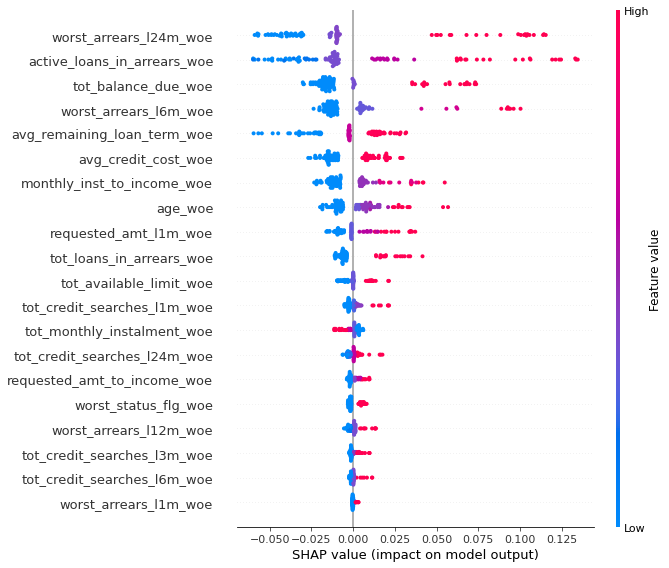
\includegraphics[width=0.8\linewidth]{Credit_Images/Sigmoid_nn_shap.png}
   \caption{Neural Network WOE with just the input layer and output sigmoid layer.}
    \label{fig-deep-shap-WOE-sig}
\end{figure}

\subsection{Attributions between normal and bias class weights}
Comparing the feature attributions between Figure \ref{fig-deep-shap-NN} and \ref{fig-deep-shap-weighted-NN}, there are a few key differences. The first is that the order of the features are different which means the features which contribute the most differ. Looking at \emph{monthly\_inst\_to\_income} and \emph{total\_loan\_in\_arrears} in Figure  \ref{fig-deep-shap-weighted-NN}, it can be seen that they have stronger attributions towards the \emph{default} class in the weighted model. Another notable difference is the \emph{worst\_arrears\_l24m\_feature}, in Figure \ref{fig-deep-shap-weighted-NN} the maximum value possible SHAP value is larger which means that this feature can have a larger effect on the models outcome. From this we can see that it seems that by using the misclassification costs introduced in Chapter \ref{sec-class-imbalance} some of the features were given more predictive power towards the \emph{default} class.

\subsection{Prediction strength relative to Feature magnitude} \label{sect-prediction-strength}
With SHAP we are able to sample the explanations over multiple instances. If the chosen background instances are diverse, we are able to view how the feature attributions react over varying magnitudes. For example if we look at the odds ratio for \emph{worst\_status\_flg} in table \ref{table:logistic} we can see that the feature has an \emph{odds ratio} of $1.069937$ which by using our domain knowledge we know that this is a binary categorical variable which can only take on a value of 0 or 1. However if we did not have domain knowledge about this variable it could possibly be mistaken as a \emph{continuous variable} which makes it seem as though it could have a much larger contribution than it actually does. Now if we compare to this to the SHAP explanation in Figure \ref{fig-deep-shap-NN} we can see how the features contributions reacts at different values. From this we can see that regardless of it's magnitude the feature relatively has the same contribution if it is high and a small contribution when it is low. It would require more effort and observing the original feature to discern this from just the Logistic Regression explanation. This could possibly be used for \emph{Feature Selection}. By observing how the contribution of a feature changes over varying magnitudes we can choose to manually remove features which regardless of their intensity seem to add little value. If we once again look at Figure \ref{fig-deep-shap-NN}, the feature \emph{tot\_monthly\_instalment} seems have a very low SHAP Value even when it's feature value is high and could possibly be considered for removal. 
 \chapter{Conclusion}
The aim for this thesis was to provide explanations into the decisions made by Neural Networks so that they may be considered as possible solutions to problems where interpretability is a strict requirement. We discuss the findings which we have gathered during this experiment and note some work that still has to be done.
\section{Conclusions}
\subsection{Explaining simple Neural Networks}
We were able to produce explanations for various different model architectures and have also proved that the explanations generated by LIME and SHAP are nearly identical to the weight coefficients extracted from linear models. We were able to deduce how much each feature contributes relative to their magnitude and to one another. Therefore we can conclude that these tools do provide interpretations into black-box networks, however we are only able to gather a simple relationship between the input and output layers, with \emph{Lucid} being the only tool which attempts to explain the relationship between hidden layers.
\subsection{Lucid is complicated to use}
From our evaluation of \emph{Lucid} we have shown that it requires considerable effort and probing into the network in order to gather any form of visualization. It is still an actively developed project and therefore there is not much documentation on how to adapt it for use with different model architectures. Although Lucid is hard to use for models which have already being built, it can be valuable while developing an image-based model to understand exactly what is happening within each layer.
\subsection{Exposing problems within the model}
As we have seen in Section \ref{sect-problem-expose} by using SHAP we were able to expose a misbehaving feature in our Neural Network. Although by simply viewing performance metrics, a model may seem to be performing well, by looking at the produced explanations we were able to notice that there was an issue either within our models architecture or the data itself. This is useful when testing whether a model is trustworthy enough to be used in production.
\subsection{Comparing network architectures}
As seen in Section \ref{sect-architecure} we were able to demonstrate how a change in a Neural Networks architecture affected the features which contribute towards the prediction. It is common when training a Neural Network to experiment with different hidden layers and activation functions. By making use of SHAP explanations this can help us identify which variations are best suited into solving our problem.
\subsection{Using SHAP for feature selection}
Looking at Section \ref{sect-prediction-strength} we have seen that by observing our SHAP explanations we were able to discover features which contribute little towards the prediction. Discovering variables with weak predictive strength was as simple as looking at how the SHAP value changed based on the features magnitude. This may be considered a manual process however it can scale well into many features, as it is ordered according to predictive strength. This can also be used when heavily correlated variables are discovered and a decision has to be made as to which to keep and which to remove.
\subsection{SHAP is in most ways superior to LIME}
Comparing the explanations of LIME to SHAP we can see that SHAP is more descriptive and provides more ways to express the explanations. The largest limitation of LIME is that it is only able to provide explanations for a single prediction at a time and the explanations provided can be seen as a local explanation. SHAP allows us to use a set of background samples where the SHAP values are calculated using all of these samples. SHAP also allows us to view explanations of multiple instances at a time in order to compare their magnitudes. This is to be expected since SHAP further expands upon the ideas introduced by LIME, therefore we are able to conclude that SHAP is the superior model agnostic explainer.
\section{Future Work}
\subsection{Complex networks}
All our experiments were based on simple architectures and therefore we do not know how well these tools scale for larger and more complex networks. Further experimentation has to be done in order to conclude that these tools are stable enough to be used for production models.
\subsection{Streamlining Lucid}
Lucid is the only tool which gains insight into the relationship of hidden layers. At the time of writing Lucid only works with Tensorflow 1 and is an extensive toolkit without much documentation on how to adapt it for use in custom models. It would be interesting to contribute to it's active research by providing functionality for platform independent Neural Networks and streamlining the process of interpretation.
\subsection{Explaining hidden layers}
Both LIME and SHAP are unable to provide insight into hidden layers which are arguably the most interesting part of Neural Networks. Further work could include adapting the concepts introduced in SHAP to be able to provide explanations between any two layers within a network.
\subsection{Fooling LIME and SHAP}
The paper \emph{Fooling LIME and SHAP: Adversarial Attacks on Post hoc Explanation Methods} \cite{slack2020fooling} provides a reason as to why the explanations of \emph{LIME} and \emph{SHAP} are not always to be trusted since they are prone to attacks by adversaries which aim to alter the produced explanations. A novel \emph{scaffolding} technique is introduced which effectively hides the bias of any given classifier. Using a real world dataset known as \emph{COMPAS} which has a inherent racist bias, the authors of the paper were able to fool LIME and SHAP into producing innocuous explanations that do not expose this bias. This is an exploit that has to be further explored and fixed before we can consider using them for models in production where they are open to attacks by adversaries.
 %==== END Evaluation Section ====================================================



% Bibliography
\bibliography{references}

\end{document}
